\documentclass[12pt,twoside,a4paper]{report}

\usepackage{amsfonts,amssymb,amsmath,epsfig}
\usepackage[portuguese,brazil]{babel}    % dá suporte para os termos na língua portuguesa do Brasil
%\usepackage[latin1]{inputenc} % dá suporte para caracteres especiais como acentos e cedilha
%\usepackage{ucs}
\usepackage[utf8]{inputenc}
\usepackage[T1]{fontenc}      % Lê a codificação de fonte T1 (font encoding default é 0T1).
\usepackage{ae}               % Fonte "Almost European"
%% \usepackage[portuguese]{babel}
%% %\usepackage[brazil,english]{babel}
%% %\usepackage[english,brazil]{babel}
%% \usepackage[T1]{fontenc}
\usepackage{indentfirst}
\usepackage{graphicx}

% ,fleqn] - Alinha as equações a esquerda ao invés de centraliza-las
%\setlength{\mathindent}{1cm} % determina o espaçamento entre a margem
                              % esquerda e as equações
                              
\usepackage{fancyhdr}
\usepackage{longtable}
\usepackage{multirow}
\usepackage[T1]{fontenc}
\usepackage{ae}
\usepackage{color}
\usepackage[printonlyused]{acronym}
\usepackage{float} %put images where they are declared
\floatplacement{figure}{H}
\usepackage{amsmath}
\usepackage{amsfonts}
\usepackage{hyperref}
\usepackage{epigraph}
\usepackage[top=3cm,bottom=3.5cm,right=2cm,left=2cm]{geometry}
%---- Tamanho das Paginas ----

%\oddsidemargin  =   2 mm
%\evensidemargin = -12 mm
%\oddsidemargin  =  -1 mm  %-5
%\evensidemargin =  -1 mm %-5
%\textwidth      = 163 mm %170
%\textheight     = 209 mm %235
%\topmargin      = 7 mm %-10
%\topskip        =  5  mm %10
%\headsep        =  6 mm %10
%\footskip       =   0 mm

%---- Espaçamento entre as linhas ----

\newcommand{\blst}{1.5} %{1.15}
\renewcommand{\baselinestretch}{\blst}

%---- Formato das Paginas ----

\pagestyle{headings}
\raggedbottom                 %  impede o ajustamento vertical

%---- Especificacoes sobre figuras ----

\setcounter  {topnumber}      {2}
\setcounter  {bottomnumber}   {2}
\setcounter  {totalnumber}    {2}
\renewcommand{\topfraction}   {1}
\renewcommand{\bottomfraction}{1}
\renewcommand{\textfraction}  {0}

%---- Formatando os títulos ----

\usepackage[bf,rm,compact]{titlesec}
\font\bigrm = cmr10 at 40pt
\titleformat{\chapter}[display]
            {\normalfont\huge\sffamily}
%            {\thispagestyle{empty}\normalfont\huge\sffamily}
            {\rightline{\normalfont\bigrm{\thechapter}}}
            {-2cm}
            {\bfseries}
            [{\vspace{-5mm}\hrulefill\\[.8ex]}]
\titlespacing{\chapter}
            {0cm}{0.0cm}{0cm}

%---- Headers ----

\usepackage{fancyhdr}
\pagestyle{fancyplain}
\renewcommand{\chaptermark}[1]{\markboth{\thechapter.\ #1}{} }
\renewcommand{\sectionmark}[1]{\markright{\thesection\ #1}}
\lhead[\fancyplain{}{\bfseries\thepage}]
       {\fancyplain{}{\small\slshape\bfseries\leftmark}}
\rhead[\fancyplain{}{\small\slshape\bfseries\rightmark}]
       {\fancyplain{}{\bfseries\thepage}}
\cfoot[\fancyplain{\bfseries\thepage}{}]
       {\fancyplain{\bfseries\thepage}{}}
\renewcommand{\headrulewidth}{0.3pt}

%---- Especificacoes Numeração ----

\setcounter{secnumdepth}{1}   %  numera apenas ate as seções
\setcounter{tocdepth}{1}      %  inclui no índice somente as seções

%%\input{hifen.tex}


\begin{document}

%%%%%%%%%%%%%%%%%%%%%%%%%%%%%%%%%
\pagestyle{plain}
%\pagenumbering{arabic}
\pagenumbering{roman}
\thispagestyle{empty}
\vspace{-5cm}

\includegraphics[width=.94\textwidth, height=1in,
keepaspectratio=true]{logos/logo_Unicamp}

\begin{center}
{\large Maria Helena Gonçalves}\\ 
\vspace{7.5cm}
{\huge Números mágicos presentes
\vspace{0.4cm}
nos espectros de massa das nanopartículas de prata}

\vspace{3.5cm}

\end{center}

\begin{center}



\vspace{2cm}

%\noindent {\Large{Orientador:} Prof. Dr. Pedro Orientador} \\


%\vspace{1cm}


%\begin{tabular}{l}

%Departamento de Física Aplicada \\
%Instituto de Física {\em Gleb Wataghin}\\
%Universidade Estadual de Campinas
%\end{tabular}

\end{center}

\vspace{2cm}

\begin{center}

\noindent {\Large{Campinas - SP}} \\
\noindent {\Large{2018}} \\

\end{center}


\pagestyle{plain}
%\pagenumbering{arabic}
%\pagenumbering{roman}
%\thispagestyle{empty}
\vspace{-5cm}

\includegraphics[width=.94\textwidth, height=1in,
keepaspectratio=true]{logos/logo_Unicamp}

\begin{center}
{\Large {\sc Universidade Estadual de Campinas \\}

Instituto de Física  Gleb Wataghin \\
\vspace{0.5cm}
}
{\Large {\Large Maria Helena Gonçalves}\\
}

\vspace{3.5cm}
{\huge Números mágicos presentes
\vspace{0.4cm}
nos espectros de massa das nanopartículas de prata}

\vspace{2.5cm}

\end{center}

\begin{flushright}
  \begin{minipage}[c]{.5\textwidth}
        Monografia, apresentada ao Curso de Licenciatura em Física da Universidade Estadual de Campinas como requisito para obtenção do título de licenciatura em Física.
        
        \vspace{.2cm}
        \textbf{Orientador:} Prof. Dr. Varlei Rodrigues
    
  \end{minipage}
\end{flushright}

\begin{center}



\vspace{1cm}

%\noindent {\Large{Orientador:} Prof. Dr. Pedro Orientador} \\


%\vspace{1cm}


%\begin{tabular}{l}

%Departamento de Física Aplicada \\
%Instituto de Física {\em Gleb Wataghin}\\
%Universidade Estadual de Campinas
%\end{tabular}

\end{center}

\vspace{1cm}

\begin{center}

\noindent {\Large{Campinas - SP}} \\
\noindent {\Large{2018}} \\

\end{center}

\newpage

$ $

\newpage

\newpage

\vspace*{\fill}

{\large \hfill Ao Mateus,}

{\large \hfill pelas transformações em mim}

\newpage

$ $

\newpage

\chapter*{Agradecimentos}

A meu orientador, Prof. Dr. Varlei Rodrigues, pela compreensão, paciência e dedicação com que orientou meu trabalho.

Ao Dr. Vitor T. A. Oiko, pelos valiosos ensinamentos no início de meu percurso dentro do grupo e pelas indicações bibliográficas.

Ao Mateus, por sua lucidez, apoio, carinho e amor  demonstrados, e também pelas incontáveis conversas filosóficas.

À minha mãe, Helena, que sempre acreditou em mim.

Ao meu amigo, Nico, pelas incontáveis risadas e idiomas desenvolvidos.

Aos amigos de laboratório por todas as discussões, conversas e risadas. Em especial ao Rafa, Malu, Murilo, Marcos, Gabriel e Diego.


\newpage
\vspace*{\fill}
\epigraph{\textit{Quem deve enfrentar monstros deve permanecer atento para
não se tornar também um monstro. Se olhares demasiado tempo dentro de um abismo,  o abismo acabará por olhar dentro de ti.}}{Friedrich Nietzsche}

%\vspace*{17cm}

%{\large \hfill \ }}
%{\large \hfill \textit{}}
%{\large \hfill (Friedrich Nietzsche)}

\newpage

$ $

\chapter*{Resumo}
\markboth{Resumo}{Resumo}
\addcontentsline{toc}{chapter}{Resumo}

\textit{Clusters}, são agregados de átomos ou moléculas que variam desde três a vários milhares átomos e possuem propriedades interessantes que os tornam diferentes quando comparados ao material massivo. Essas propriedades dependem fortemente do tamanho e das estruturas geométricas que os compõem. Isso decorre dos efeitos entre a razão do número de átomos presentes na superfície e o número de átomos no
volume, ademas dos níveis  de energia discretos. Com o objetivo de melhor entender essas propriedades, faz se necessário o estudo e compreensão da estabilidade dessas estruturas. Em um artigo publicado por Knight \cite{electronic_Shell_sodium}, medidas da distribuição de massas de \textit{clusters} de sódio ($Na$), mostram picos bem definidos e visivelmente maiores que os demais, para \textit{clusters} com $2, 18, 20, 34, 40, 58,92 ...$ átomos. Esses picos dizem respeito à maior abundância e estabilidade dos \textit{clusters} atômicos desses tamanhos em relação aos demais. Estes foram apelidados de "\textit{clusters} com números
\textit{mágicos} de átomos", cujos padrões foram atribuídos aos efeitos de preenchimento das camadas eletrônicas \cite{Brack}. Com intuito de observar e entender melhor esses padrões para os \textit{clusters} de prata, foram realizados experimentos, com incidência de luz ultravioleta e sem a iluminação, para que fosse possível comparar os espectros  de abundância obtidos. Com isso foi possível estudar as tendências da abundância da formação dos \textit{clusters} de prata de diversos tamanhos e correlacionar com sua propriedades estruturais. Os picos mais energeticamente estáveis foram indicados pelos picos iguais à $n= 3,9,21,35...$ átomos, devido ao caráter iônico das partículas produzidas no experimento. Além disso, os números mágicos também poderiam decorrer do potencial de ionização dos agregados, porém isso não foi observado. Outro fato que tornou-se evidente com a realização dos experimentos foi a mudança na intensidade dos picos quando o LED encontra-se ligado e quando o LED encontra-se desligado; no primeiro caso   temos uma intensidade dos picos muito maior.

\newpage

$ $
\newpage

\chapter*{Abstract}
\markboth{Abstract}{Abstract}
\addcontentsline{toc}{chapter}{Abstract}

In the first part 


%\newpage

\chapter*{Biografia do Autor}
\markboth{Biografia do Autor}{Biografia do Autor}
\addcontentsline{toc}{chapter}{Biografia do Autor}

Concluí a escola média em 2010. Durante quatro anos trabalhei como webmaster
na empresa XXX, onde .... Iniciei o curso de física em 2013. Em 2015 como
aluno de iniciação científica e orientação do prof. Pedro Orientador
iniciei o desenvolvimento do projeto ... No final deste curso pretendo
buscar uma colocação em uma instituição financeira a fim de realizar
simulações de interesse no mercado acionário.

\newpage

$ $



\newpage

\pagestyle{fancyplain}

\tableofcontents
%%%%%%%%%%%%%%%%%%%%%%%%%%%%%%%%%

%%%%%%%%%%%%%TEXTO%%%%%%%%%%%%%%%

\chapter{Introdução}
\pagenumbering{arabic}

A partir do fim da década de 70, os estudos de estruturas nanométricas começaram a ganhar destaque por sua relevância para a área da biomedicina. Duas décadas depois, o interesse em nanossistemas também ganhou força na área da física e desde então, os estudos nessa área cresceram em ritmo acelerado. As nanoestruturas apresentam propriedades novas e interessantes que as diferem enormemente dos sistemas macroscópicos e possuem com grande potencial tecnológico em áreas como: química \cite{catalise}, eletrônica \cite{semicondutores} e biomedicina \cite{antimicrobial_effects, drug_delivery}.


Neste contexto, os nanoagregados (ou \textit{clusters} atômicos), são um caso interessante, pois podem ser compostos de três a vários milhares de átomos, podendo ser formados por um ou mais elementos, e encontram-se na fronteira entre entre a física atômica e a física da matéria condensada.
%os átomos e o \textit{bulk}\footnote{\textit{Entende-se como "bulk" um conjunto de partículas sólidas grande o suficiente para que a média estatística de suas propriedades seja independente do número de partículas\cite{bulk}}}.
Seu estudo possibilita uma melhor compreensão de como as propriedades macroscópicas surgem do comportamento quântico da matéria \cite{Heer,Brack}.

As propriedades físico-químicas das nanopartículas podem variar de forma abrupta com seu tamanho, principalmente quando se trata de \textit{clusters} atômicos, cujo diâmetro varia até \mbox{1 nm}. Esse fato implica que é possível controlar essas propriedades se seu processo de formação for precisamente controlado  \cite{energetic_thermodynamic}, o que fomenta ainda mais o potencial tecnológico dessas estruturas.


Assim, uma das vertentes dos estudos realizados pelo Grupo   de   Física   de   Nanossistemas   e Materiais  Nanoestruturados  (GFNMN)  do  Departamento de  Física  Aplicada  (DFA),  são nanopartículas metálicas produzidas por uma Fonte de \textit{Clusters} e Agregados (FoCA). Este instrumento produz nano-partículas por um método físico, com controle de seu tamanho e de sua dispersão, além da sua composição. A FoCA foi desenvolvida por Artur Domingues Tavares de Sá e Giulia Di Domenicantonio \cite{tese_artur}, ex-membros do grupo, para possibilitar o estudo mais aprofundado das nanoestruturas.

Para obter a análise de distribuição de tamanho dos \textit{clusters}, por meio da distribuição de massa dessas partículas, é utilizado a técnica de espectrometria de massa por tempo de voo, possibilitando, assim, um estudo sobre suas propriedades em função do tamanho das partículas, o que torna a utilização dessa máquina muito interessante para o grupo.

% Esse tipo de análise permite que seja estudado critérios fundamentais para as tendências estruturais e energéticas.

Em um artigo seminal publicado por Knight \textit{et. al.} \cite{electronic_Shell_sodium}, medidas da distribuição de massas de \textit{clusters} de sódio, produzidos em fase gasosa, mostram picos bem definidos e visivelmente maiores que os demais, para \textit{clusters} com $2, 18, 20, 34, 40, 58,92 ...$ átomos. Esses picos dizem respeito à maior abundância e estabilidade dos \textit{clusters} atômicos desses tamanhos em relação aos demais. Apelidou-se a esses \textit{clusters} de "\textit{clusters} com números
\textit{mágicos} de átomos", cujos padrões foram atribuídos aos efeitos de preenchimento das camadas eletrônicas \cite{Brack}. O modelo quântico de Jellium \cite{jellium} obteve sucesso para explicar os números \textit{mágicos}, mas também existem casos em que \textit{clusters} com número \textit{mágicos} átomos também aparecem devido ao preenchimento de camadas geométricas ou poliédricas, deixando de ser uma propriedade eletrônica.


Os números mágicos não aparecem somente para o elemento sódio, mas sim para uma série de elementos incluindo os metais de transição como \cite{magic_1B}  cobre, prata, ouro, platina, dentre muitos outros.

Um dos objetivos desse trabalho é utilizar a Fonte de \textit{Clusters} e Agregados e a técnica de espectrometria de massa por tempo de voo para estudar as tendências da abundância da formação dos \textit{clusters} de diversos tamanhos e correlacionar com sua propriedades estruturais e energéticas. Pretende-se realizar experimentos com um metal de transição - no caso prata - para verificar o aparecimento dos \textit{clusters} com números \textit{mágicos}. Além disso, os números mágicos também ocorrem no potencial de ionização dos agregados. Assim, pretendemos realizar experimentos com incidência de luz ultravioleta (UV), induzindo a sua ionização, e comparar os espectros de abundância obtidos com e sem o uso da luz UV. 

No capítulo 2 deste trabalho, serão  abordados os embasamentos teóricos sobre o aparecimento dos \textit{clusters} com números \textit{mágicos} sustentado pela literatura disponível. Subsequentemente, no capítulo 3 apresentaremos a máquina utilizada para a produção de \textit{clusters} e as modificações feitas na máquina para conseguir realizar os experimentos com luz UV. Discutiremos no capítulo seguinte as caracterizações
realizadas da prata e os resultados obtidos. Por fim, realizaremos um
compêndio geral do trabalho apresentado, mostrando as principais conclusões. 



 
\chapter{Revisão Bibliográfica}
\label{revisao_bibliografica}

\section{Clusters}
\label{c2-clusters}

\textit{Clusters} são agregados de átomos ou moléculas, que variam desde dois a vários milhares de átomos e encontram-se na fronteira entre os átomos e o \textit{bulk}\footnote{\textit{Entende-se como "bulk" um conjunto de partículas grande o suficiente para que a média estatística de suas propriedades seja independente do número de partículas\cite{bulk}}}\cite{Heer,Brack}, por definição, eles se encontram em uma escala nanométrica ($ \leqslant 100$ nm).
No geral, os \textit{clusters} atômicos são classificados de acordo com seu tamanho: \textcolor{blue}{ muito pequenos, pequenos, médios ou grandes. Aglomerados classificados como muito pequenos e pequenos apresentam propriedades quânticas e possuem uma grande dependência com número de partículas que o compõe, essas propriedades não variam suavemente com seu tamanho, diferentemente dos \textit{clusters} médios e grandes.
Normalmente os \textit{clusters} são classificados pelo números de àtomos(n) que o compõem: muito pequenos ($3<n<12$), pequenos($13<n<100$), médios ($100<n<1000$) e grandes ($1000<n<10^8$).}
\textcolor{red}{Normalmente os \textit{clusters} são ditos pequenos quando contém da ordem de centas a mil partículas} Os nano-agregados considerados grandes possuem propriedades tendem a seguir as propriedades da matéria um \textit{bulk}.


Deixando de lado os casos limites que geram ambiguidades, a diferença entre \textit{cluster} e moléculas encontra-se no fato que estas, no geral, possuem composições específicas e bem definidas e, na grande maioria dos casos, suas estruturas também são bem definidas, tendo  assim um número restrito de átomos; diferente de um \textit{cluster} que, como exemplo, podemos citar um \textit{cluster} de prata que pode conter de 2, 15, 100, a qualquer número de átomos de prata, respeitando os limites impostos para que este ainda seja um \textit{cluster}. Esses, por sua vez, também não possuem uma estrutura única, como podemos ver na Figura \ref{fig:estrutura_cluster_ag}, e para sua maioria, à medida que o número de partículas do \textit{cluster} aumenta, o número de estruturas estáveis disponíveis torna-se mais abundante. 

\begin{figure}
  \centering
  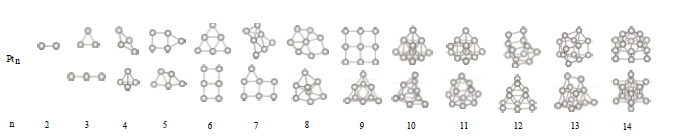
\includegraphics[width=1\textwidth]{images/clusters/estrutura_cluster_ag}
  \caption{ Exemplo de estruturas de \textit{clusters} de prata.\cite{dissertacao_anderson}  }
  \label{fig:estrutura_cluster_ag}
\end{figure}


 A análise das estruturas dos \textit{clusters} é fundamental para compreender suas propriedades e  dispor de seus potenciais tecnológicos, isso também torna-se muito importante para o domínio da estabilidade das nanopartículas. 


A análise da distribuição do tamanho dos \textit{clusters} pode prover critérios fundamentais para o entendimento das tendências estruturais e energéticas dos mesmos. Buscando entender melhor as transições das propriedades dos \textit{clusters}, segundo Bernd v. Issendorff (2009), podemos começar os estudos pensando em uma descrição simples, porém suficiente, do modo como se comportam os elétrons de um metal. Assumindo um sistema de elétrons livres, isto é, cujos elétrons da camada de valência se movem através de uma rede de metal infinita, agindo como partículas livres. Assim, as funções de onda eletrônicas são apenas ondas planas, tornando qualquer comprimento de onda possível.

Mudanças significativas ocorrem quando o metal possui dimensões nanoscópicas ou são nanopartículas. Agora, as funções de onda formam ondas estacionárias entre as superfícies da partícula, o que é possível somente para certos comprimentos de onda. Uma consequência direta é a discretização da densidade eletrônica de estados: a banda de valência contínua se divide em um número finito de estados. Este é o chamado efeito de tamanho, um efeito quântico que pode levar a mudanças significativas nas propriedades das partículas de metal. Pode-se esperar que tais efeitos possam ser mais claramente vistos para um metal que se aproxime do comportamento ideal dos elétrons livres \cite{capitulo_livro_shell}.

A Figura \ref{fig:transicao_cluster_solido} mostra a mudança das propriedades de um material enquanto \textit{clusters} e enquanto sólido massivo. \textcolor{blue}{Note que, as propriedades enquanto átomos ou moléculas que se comportam como \textit{clusters}, são não monotônicas, enquanto que apartir dos \textit{clusters} que se comportam como sólidos, as propriedades são monotônicas. Na região em que temos um regime de propriedades não monotônicas, propriedades incomuns para certos tipos de material podem surgir devido ao do confinamento quântico e dos efeitos de contorno. \textit{Clusters} de elementos não magnéticos tornam-se magnéticos, materiais semicondutores exibem propriedades metálicas, sistemas metálicos tornam-se semicondutores, a cor de partículas muda com tamanho, metais nobres tornam-se reativos e materiais frágeis tornam-se maleáveis.}\textcolor{red}{não dá para entender a relação do texto e a figura. Precisa falar da variação das propriedades monotônicas e não monotônicas}

\begin{figure}
  \centering
  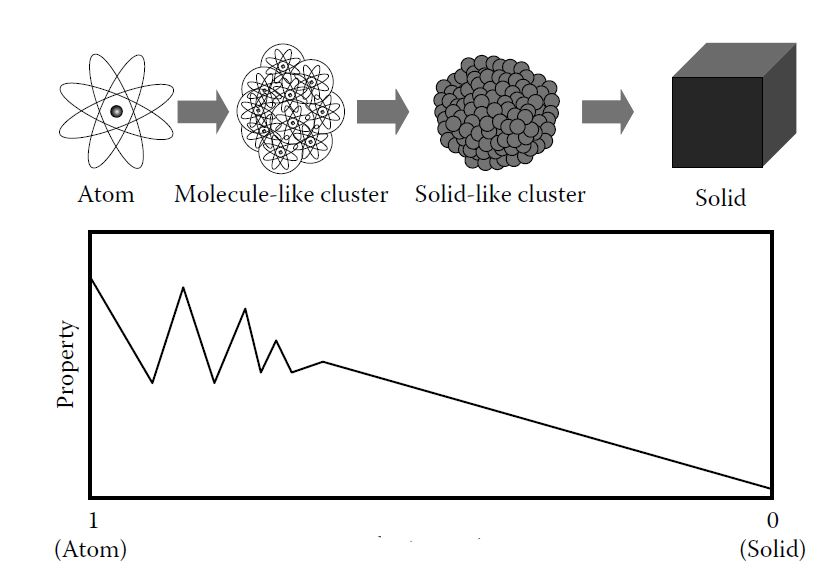
\includegraphics[width=0.7\textwidth]{images/clusters/atomo_cluste_solido}
  \caption{Esquema de transformação dimensional de átomos através de pequenos e grandes \textit{clusters} para o estado sólido. Quando os \textit{clusters} são pequenos cada átomo adicionado é importante, por isso as propriedades mudam
de forma abrupta com o tamanho. Quando os \textit{clusters} se tornam grandes,
propriedades mudam suavemente\cite{cap06_Nanophysics}. Adaptado.  }
  \label{fig:transicao_cluster_solido}
\end{figure}


Os estudos sobre as propriedades das nanopartículas indicam que a banda de condução eletrônica contínua de um sólido se divide em estados discretos se o metal for suficientemente pequeno. Para \textit{clusters} considerados grandes, a quantidade de níveis aumenta enquanto a largura do \textit{gap} diminui, levando à estrutura de banda do bulk.

Uma das mudanças de propriedade interessantes de serem estudadas é a função dielétrica do material. Quando os \textit{clusters} metálicos são considerados pequenos, a banda de condução se divide em níveis discretos separados por energias $\sigma$, que são maiores quando comparadas com as energias térmicas, sendo assim $\sigma>kT$, como pode-se ver na Figura \ref{fig:carac_metal}. Isso indica que as nanopartículas podem ter propriedades semelhantes a semicondutores, se aumentarmos um pouco seu tamanho, essas começaram a exibir comportamentos de pequenos pedaços do metal macroscópico.

\begin{figure}
  \centering
  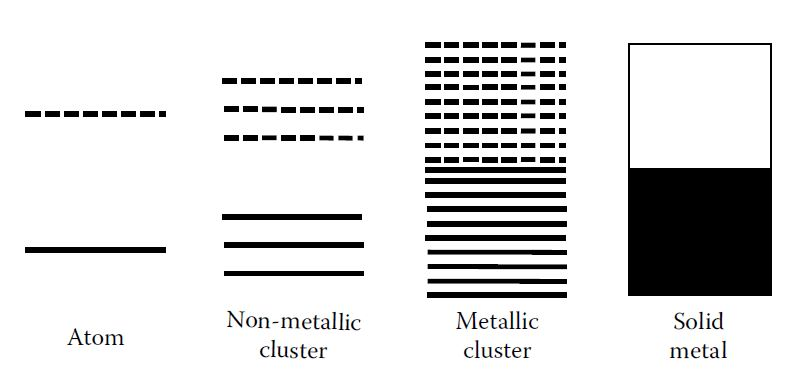
\includegraphics[width=0.65\textwidth]{images/clusters/carac_metal}
  \caption{ Esquema de transformação estrutural de energia desde de átomos de metal, pequenos e grandes \textit{clusters}, até o metal sólido. Abaixo de um certo tamanho de \textit{cluster}, no qual as bandas vazia e povoada se fundem, um \textit{cluster} de átomos de metal pode ter uma estrutura de energia semelhante a um semicondutor.\cite{dissertacao_anderson}  }
  \label{fig:carac_metal}
\end{figure}

Os \textit{clusters} podem ser produzidos a partir de diversos elementos da tabela periódica, como, por exemplo, metais alcalinos como sódio e potássio; metais alcalinos-terrosos, como cálcio, magnésio e bário; metais nobres, como ouro, prata  e cobre. Quando estudadas as nanopartículas de materiais que pertencem à mesma família, suas propriedades seguem o mesmo padrão.


\section{Espectro de massa das nanopartículas}
\label{sec:experimentos_teo}


Em 1984, Knight et al \cite{electronic_Shell_sodium} realizou um experimento com nanopartículas de sódio, com N átomos por conglomerado (N = 4-100), e foram encontrados padrões, com picos bem definidos, no espectro de massa de \textit{clusters} de Na em fase gasosa, podendo ser visto na Figura \ref{fig:espec_na}(a). Cada pico do espectro representa o número de 
aglomerados de um determinado N detectado. Note a presença de picos maiores, quando comparado com os outros picos, para certas massas correspondentes a N = $8, 20, 40, 58$ e $92$, onde podemos notar padrões. 




\begin{figure}
  \centering
  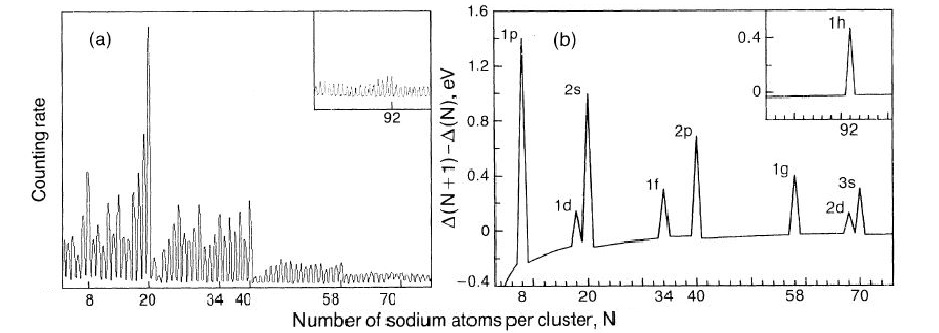
\includegraphics[width=1\textwidth]{images/clusters/NA_knight}
  \caption{(a) Espectro de massa de \textit{clusters} de sódio, N = 4-75.
  (b) A mudança calculada na diferença de energia eletrônica. Os picos protuberantes correspondem aos orbitais de casca fechada.\cite{electronic_Shell_sodium}  }
  \label{fig:espec_na}
\end{figure}


As características dos espectros de massa de outros metais alcalinos, e também dos metais nobres, seguem um padrão semelhante ao do sódio.

Em 1985, Katakuse et al \cite{KATAKUSE1985229} realizou um experimento com nanopartículas de cobre, prata e ouro, com $250$ átomos, e também foram encontrados padrões, com picos bem definidos em cada espectro de massa, como podemos ver nas Figuras \ref{fig:espec_ag},\ref{fig:espec_cu} e \ref{fig:espec_au}. No espectro de prata , podemos notar uma maior abundância nos picos como número de átomos iguais, $n= 3,9,21,35,41,59,93,139$ e $200$, já no espectro de cobre vemos que a abundância dos picos são nos \textit{clusters} com $n= 3,9,21,35,41,59,93,139$ e no espectro de ouro vemos que a abundância dos picos são nos \textit{clusters} com $n= 3,9,21,35,59,93,139$. \textcolor{blue}{Essa diferença ocorre devido as nanopartículas de prata, cobre e ouro serem ionizadas contendo um elétron a mais; como exemplos podemos citar o \textit{cluster} de prata 9:
\begin{equation*}
    Ag_{9} \to Ag_{8} + e^{-}
\end{equation*}} \textcolor{red}{Precisa explicar porque 3, 9, 21, ... ao invésde 2, 8, 20, ....}






\begin{figure}
  \centering
  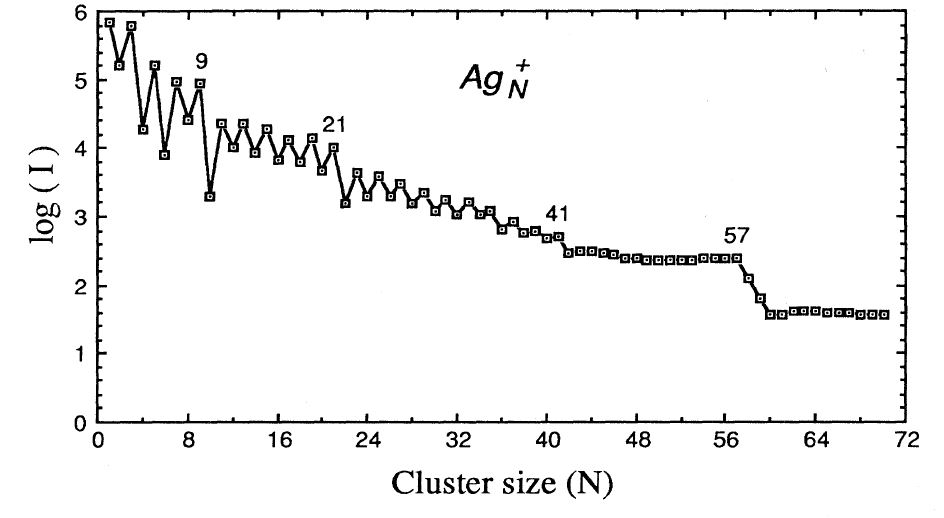
\includegraphics[width=0.7\textwidth]{images/clusters/espec_ag}
  \caption{(a) Espectro de massa de \textit{clusters} de prata \cite{Heer}.  }
  \label{fig:espec_ag}
\end{figure}

\begin{figure}
  \centering
  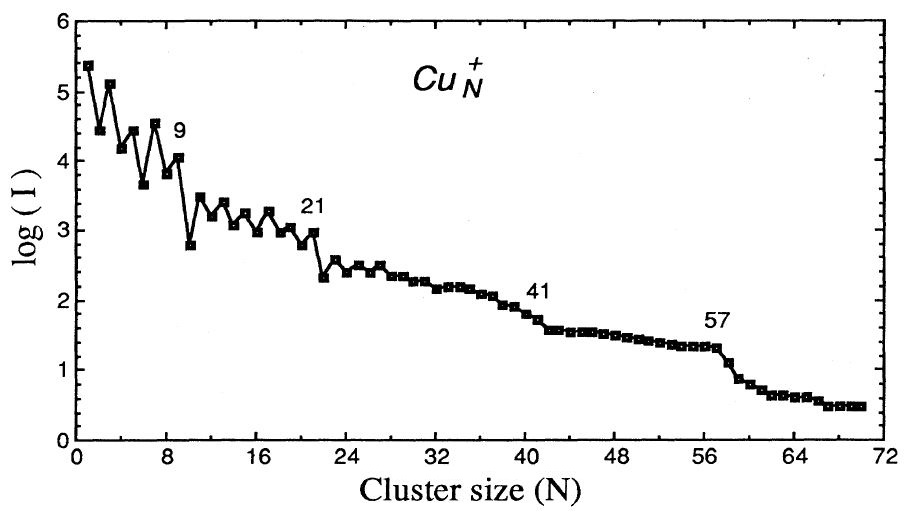
\includegraphics[width=0.7\textwidth]{images/clusters/espec_cu}
  \caption{(a) Espectro de massa de \textit{clusters} de cobre \cite{Heer}.  }
  \label{fig:espec_cu}
\end{figure}

\begin{figure}
  \centering
  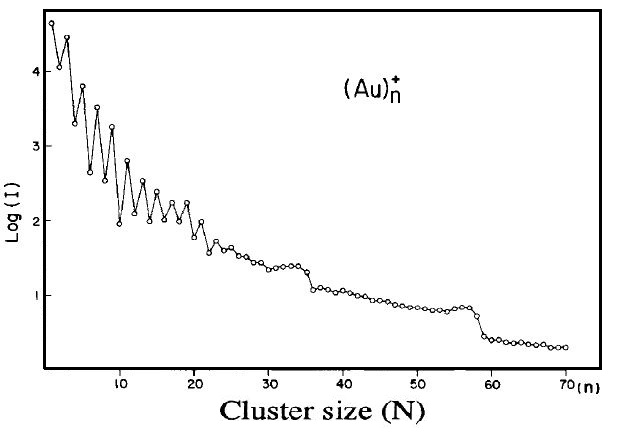
\includegraphics[width=0.65\textwidth]{images/clusters/espec_au}
  \caption{(a) Espectro de massa de \textit{clusters} de ouro \cite{KATAKUSE1985229}.  }
  \label{fig:espec_au}
\end{figure}




Os \textit{clusters} mais abundantes
nos espectros de massa foram apelidados de \textit{clusters mágicos}, ou \textit{clusters com números mágicos de átomos}, e são considerados relativamente mais estáveis. Podemos destacar a estrutura eletrônica dessas nanopartículas como a causa de maior estabilidade, como veremos a seguir.

Para explicar a ocorrência desses \textit{clusters mágicos}, foi suposto o efeito de preenchimento de camadas eletrônicas em que a combinação entre o espectro de estados
quantizados e o princípio de exclusão de Pauli resultam em efeitos de camada \cite{Brack}, ou seja, $1s^{2}$, $1s^{2}1p^{6}$, $1s^{2}1p^{6}1d^{10}$, $1s^{2}1p^{6}1d^{10} 2s^{2}$, … totalizando os números característicos do espectro de sódio mostrado na Figura \ref{fig:espec_na}. O modelo quântico de \textit{Jellium} \cite{Heer}, foi usado com sucesso para explicar a ocorrência desses \textit{clusters mágicos} \cite{capitulo_livro_shell}, como veremos na secção \ref{section_shell_model}.

Para as nanopartículas consideradas grandes, o padrão de números mágicos aparece diferente e, no geral, ele é atribuído como uma consequência do preenchimento de camadas geométricas ou poliédricas de casca, assim o \textit{cluster} assume geometrias que minimizam a relação átomo-superfície, uma vez que os átomos da superfície possuem um número menor de vizinhos do que os átomos internos, e o \textit{cluster} tende a preferir a estrutura de menor energia, maximizando a fração de átomo \textcolor{red}{em massa ?????}. Essa estrutura geométrica da \textcolor{red}{casca} é bem conhecida nos \textit{clusters} de gás, e é característica de interações de curto alcance nas quais a \textcolor{red}{tendência é o empacotamento do próximo do atomo juntamente - vamos conversar sobre essa parte} com a necessidade de minimizar a energia superficial \cite{capitulo_livro_shell}.


\section{Estrutura eletrônica \textit{shell model} para \textit{clusters} esféricos} \label{section_shell_model}

\textcolor{red}{melhorar esta frase} Pretendemos apresentar uma visão geral das características do sistema eletrônico \textit{shell model}.

O espectro de massa da \ref{fig:espec_na} sugere que os elétrons de valência nos \textit{clusters} de sódio são independentes e estão confinados em um potencial esfericamente simétrico. Assim como os átomos, com todas suas camadas eletrônicas preenchidas, as camadas eletrônicas de um \textit{cluster} com um número exato de elétrons para formar uma \textcolor{red}{estrutura geométrica poliédrica fechada} o torna muito estável. Quando um átomo for adicionado à nanoestrutura, seu elétron de valência ocupará um estado com energia maior e, assim, a estabilidade do \textit{cluster} será reduzida, reduzindo sua sua abundância no espectro, explicando a grande abundância após cada número de fechamento da camada. \cite{capitulo_livro_shell}.

Os números quânticos dos \textit{cluster} metálicos são caracterizados de modo que cada camada possui um número quântico radial \textit{n} e o momento angular \textit{l}. Para um dado número quântico \textit{l}, o estado mais baixo tem $n = 1$, e assim por diante \textcolor{red}{completar! ou retirar.}.


Uma primeira aproximação com abordagem quântica é o "Modelo de \textcolor{red}{melhor usar o jargão} Gota", que fornece uma descrição boa do comportamento observado na Figura \ref{fig:espec_na}. O \textit{cluster} é representado como uma esfera de raio \textit{R}, que está relacionada com número \textit{N} de átomos e o raio de Wigner-Seitz, $r_{s}$\cite{capitulo_livro_shell}\cite{livro_cap16_Misra2012527}.


\begin{equation}
\label{eq:raio_R}
    R = r_{s}(N)^{\frac{1}{3}}
\end{equation}

\textcolor{red}{O raio de Wigner-Seitz, $r_{s}$, é definido como o raio do volume ocupado por cada elétron de valência, que é equivalente ao volume ocupado por cada átomo em um metal monovalente.}
A estrutura interna do \textit{cluster} não é levada em consideração neste modelo, sendo ela equivalente à teoria de elétrons livres em sólidos. No entanto, a caixa sólida tem dimensões macroscópicas e níveis energéticos contínuos, enquanto o modelo para o \textit{cluster}, situado em nanoescala, os níveis de energia são discretos. Os primeiros níveis de energia para elétrons que não interagem em uma caixa esférica e o número de elétrons necessário para o preenchimento completo das camadas é $n= 2,8,18,20,34,40,58$ \cite{livro_cap16_Misra2012527}. Note que esses números condizem com os picos de maior abundância apontados no espectro da Figura \ref{fig:espec_na}.






Para o modelo de concha esféricas, os núcleos iônicos são substituídos por carga positiva uniforme de raio \textit{R}, os elétrons são tratados como partículas livres, movendo-se em um potencial parametrizado. O parâmetro básico do modelo é o raio de Wigner-Seitz, e a função onda para um potencial esfericamente simétrico pode ser escrita como:

\begin{equation}
    \psi_{ n,l,m}(r, \theta, \phi) = R_{nl}(r)Y_{lm}(\theta, \phi)
\end{equation}

Existem três potenciais úteis para o estudo da física de \textit{cluster}: potencial do oscilador harmônico, potencial esférico de poço quadrado e potencial Woods-Saxon. Estes potenciais são mostrados graficamente na Figura \ref{fig:pocos}. \textcolor{red}{A figura ficou muito longe.}

\subsubsection{Potencial do Oscilador Harmônico:}

O potencial mais simples é o potencial do oscilador harmônico $V_{r}$:

\begin{equation}
    V(r)= \frac{1}{2}m\omega_0r^2
\end{equation}

\noindent
o potencial do poço \textcolor{red}{quadrado esférico (constante para $r<R$ e infinito para os demais)}. Como podemos ver na primeira coluna da Figura \ref{fig:pocos}, os níveis de energia para o potencial do oscilador harmônico são igualmente espaçados, altamente degenerados  \textcolor{red}{e são rotulados pelo número quântico \textit{v}}.


A energia do potencial do oscilador harmônico é dada por:

\begin{equation}
    E_{v}= \left(\frac{3}{2}+v\right)h\omega_0
\end{equation}

Os números quânticos $(n,l)$ podem ser usados para qualquer potencial esfericamente simétrico. Assim, todos os orbitais com o mesmo valor de $(2n+l)$ são degenerados e as energias são escritas em termos do único número quântico $(2v+l-2)$ \textcolor{red}{que é?}. A energia potencial devido à carga de fundo é \cite{livro_cap16_Misra2012527}:
\begin{equation}
    \hbox{V}(r)
= \left\{ \begin{array}{lll}
\frac{3e^2N}{8\pi\epsilon_0R^3}\left(\frac{r^2}{3}-R^2\right) & \hbox{se} & r<R \\
e^2 Z & \hbox{} &  \\
\frac{e^2N}{4\pi\epsilon_0r} & \hbox{se} & r > R
\end{array}\right.
\end{equation}

\subsubsection{\textcolor{red}{Potencial Esférico de Poço Quadrado:}}

O potencial esférico de poços quadrados é descrito por:



\begin{equation}
 V(r) = \left\{\begin{array}{lll}
C & \hbox{se} & r < R \\
\infty & \hbox{se}  & \forall r
\end{array}\right.
\end{equation}



\noindent
em que C é uma constante. A função de onda radial $R_{nl}(r)$ para o potencial do poço quadrado é escrita em termos da função de Bessel esférica $j_{l}(K_{nl}R)$, em que

\begin{equation}
    K_{nl}=\left[\frac{2m|E|}{\hbar^2}\right]^{\frac{1}{2}}
\end{equation}

Os níveis de energia são determinados pelas condições de contorno $j_{l}(K_{nl}R)=0$ e, para cada $l$, o primeiro zero de $j_l$ é dado o número quântico $n = 1$, o segundo $n = 2$, e assim por diante. A ordem dos níveis de energia (que são emprestados da física nuclear e são diferentes da física atômica) são $1s$, $1p$, $1d$, $2s$, $1f$, $2p$, $1g$, $2d$,... Se duas soluções tiverem o mesmo número de nós radiais, aquela com maior $l$ terá maior energia. Nessa notação, o número quântico principal em física atômica é igual a $n + l$. O interior do \textit{cluster} será eletricamente neutro se incluirmos a contribuição da correlação de troca para o potencial eletrostático dos elétrons, e o potencial efetivo será quase constante. \textcolor{red}{O potencial do poço quadrado representa essencialmente esse fenômeno} \cite{livro_cap16_Misra2012527}.


\subsubsection{Potencial de Woods–Saxon:}

Em seu artigo, Knight et al\cite{electronic_Shell_sodium} utiliza o potencial de Woods-Saxon para realizar a análise dos espectros de massa de sódio mostrados na Figura \ref{fig:espec_na}\cite{livro_cap16_Misra2012527}, uma vez que ele é o potencial que melhor produz uma representação fenomenológica um potencial plano no centro de \textit{cluster} arredondado nas bordas. Este potencial é descrito por:

\begin{equation}
    U(r)=\frac{-U_0}{exp[(r-R)/\epsilon]+1}
\end{equation}


$U_0$ é a soma da energia de Fermi e a função de trabalho do metal a \textcolor{red}{granel}. $R$ é determinado pela equação \ref{eq:raio_R}. O parâmetro $\epsilon$ é usado para corresponder à variação do potencial na superfície. Para este potencial, não existem soluções analíticas.


Uma comparação entre os três potenciais apresentados pode ser vista na Figura \ref{fig:pocos}. Nela podemos ver que a degenerescência dos estados do potencial Woods-Saxon é semelhante a do potencial do poço quadrado, mas a ordenação dos níveis de energia são diferentes.

 Note também que os níveis com o mesmo momento angular são interligados. Pode-se ver que a sequência de níveis depende do potencial radial. Isso influi nos números “mágicos”, ou seja, nos números de elétrons para os quais os \textit{clusters} são especialmente estáveis. Nos níveis, os números de elétrons são: 2 elétrons preenchem o nível $1s$, 8 elétrons preenchem as camadas $1s$ e $1p$ e assim por diante.
 
 Os \textit{clusters} mais estáveis são aqueles com um nível completamente preenchido (chamado de casca fechada) e um grande espaço entre o nível ocupado mais alto e o nível mais baixo não ocupado. Portanto, os números de elétrons $34$ e $58$ são números “mágicos” do potencial quadrado, mas não do potencial Woods–Saxon. Os números $20$ e $40$ são fortemente “mágicos” para o oscilador harmônico e o potencial Woods–Saxon, mas menos para o potencial da caixa. Então, quais tamanhos de \textit{clusters} são especialmente estáveis depende fortemente do potencial radial, que pode ser diferente para diferentes metais.
 
Os números observados para 
\textit{clusters} de sódio na Figura \ref{fig:espec_na} $(8, 20, 40, 58)$ indicam que o potencial efetivo de partícula única está entre uma caixa e um potencial Woods–Saxon. Mas o mais importante é o acordo desses números com as previsões do modelo simples, o modelo de elétrons livres é capaz de descrever sistema eletrônico de \textit{clusters} de sódio \cite{livro_Clusters_Fullerenes}.

\begin{figure}
  \centering
  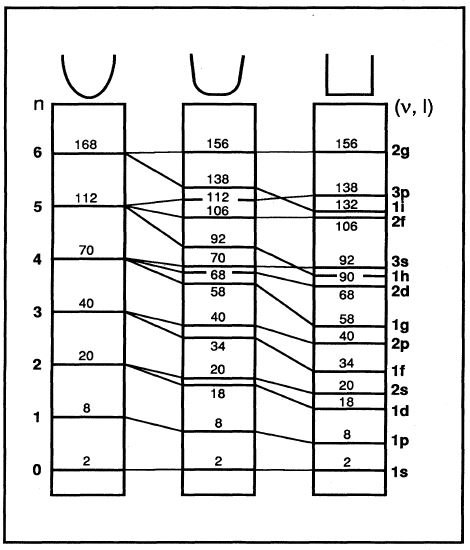
\includegraphics[width=0.5\textwidth]{images/clusters/pocos}
  \caption{Comparação dos potenciais (a) harmônico, (b) Woods-Saxon e (c) poço quadrado. \cite{Heer}}
  \label{fig:pocos}
\end{figure}

Em contrapartida, os "números mágicos"\ para os espectros de prata, cobre e ouro, mostrados nas Figuras \ref{fig:espec_ag},\ref{fig:espec_cu} e \ref{fig:espec_au}, ocorrem em
$9, 21, 35,...$ , diferente dos \textit{clusters} de sódio. Eles possuem as camadas 3d, 4d e 5d, com a camada d preenchido com 10 elétrons e um único elétron de valência. No experimento de Katakuse et. al. 1985,  os \textit{clusters} foram produzidos carregados positivamente e, assim, o número de elétrons em um aglomerado era $N - 1$, desta forma os números mágicos correspondentes às cargas eletrônicas de conchas estão coerentes com os resultados experimentais \cite{Heer}.

Comparando os espectros de sódio com os espectros dos metais nobres apresentados, vemos que neles a estrutura fina é dominada por um alternância par-ímpar nas intensidades, enquanto o espectro de sódio reflete a estrutura da subcamada prevista neste modelo. 





\chapter{Materiais e Métodos}
\label{materiais_e_metodos}

Neste capítulo serão apresentados os materiais e metodologia utilizados. Nas seções \label{sec:producao_cluster} e \ref{sec:foca}, apresentaremos
o método de síntese das nanopartículas utilizado, iniciando por uma descrição breve do tipo de síntese, seguindo com o aparato experimental utilizado neste trabalho. A seção \ref{sec:tof} apresentará a técnica de \textit{Time-of-flight Mass Spectrometers} (TOFMSs), utilizada para obter os espectros das partículas. Por fim, na seção \ref{sec:led} descreveremos o processo utilizado para iluminação dos \textit{Clusters} com luz ultravioleta.


\section{Produção \textit{Clusters}}
\label{sec:producao_cluster}

Nesta seção apresentaremos os métodos de síntese das nanopartículas.

A produção de \textit{clusters} é feita basicamente por duas técnicas: \textit{top-down} e \textit{bottom-up}. Na primeira, a partir de um material com dimensões macroscópicas, as nanoestruturas são formadas pela remoção de material utilizando técnicas como feixe de elétrons ou litografia de feixe de íons focalizado. Na segunda técnica, as nanopartículas são produzidas pela agregação de elementos básicos como átomos e moléculas. Isso ocorre por via química ou física.

Na estratégia \textit{bottom-up}, a produção de nanopartículas por via química é mais simples, porém o controle de pureza e tamanho tornam-se mais complicados. O método de produção por via física requer o uso de um aparato experimental sofisticado, como o que será apresentado neste capítulo na seção \ref{sec:foca}, porém o controle de pureza e tamanho dos \textit{clusters} são altamente precisos. Como exemplo de produção por método físico, em um caso mais geral de metais, podemos citar a evaporação térmica e a técnica de \textit{sputtering} (ou pulverização catódica).

%%%%%%%%%%%%%%_FOCA_%%%%%%%%%%%%%%%
\section{A Fonte de \textit{Clusters} e Agregados}
\label{sec:foca}
Nesta seção apresentaremos o método de síntese das nanopartículas utilizado e desenvolvido pelo grupo GFNMN.


A Fonte de \textit{Clusters} e Agregados (FoCA), esquematizada na Figura \ref{fig:esquema_foca}, produz nanopartículas metálicas que variam desde $1$ e podem chegar até à $40.000$ átomos (uma partícula de $5nm$ de diâmetro no caso da prata), sendo essa produção por método físico, mais especificamente \textit{sputtering}.

O funcionamento da máquina ocorre basicamente em quatro etapas: primeiramente uma nuvem de átomos é produzida por um \textit{sputtering}; em seguida, são resfriadas por nitrogênio líquido ocorrendo a agregação dos átomos em nanopartículas na presença do gás argônio; na sequência, o feixe de agregados, carregados eletricamente, é guiado por um conjunto de lentes eletrostáticas até chegar no espectrômetro de massa por tempo de voo, onde aproximadamente $10\%$ do feixe é desviado para a análise do espectro de distribuição de massa, sendo possível identificar a massa e, por consequência, o tamanho das partículas produzidas, que será melhor explicado na seção \ref{sec:tof}. Por fim as nanopartículas são depositadas no porta amostras. Na Figura \ref{fig:foto_foca} podemos ver uma foto real da máquina. 

\begin{figure}
  \centering
  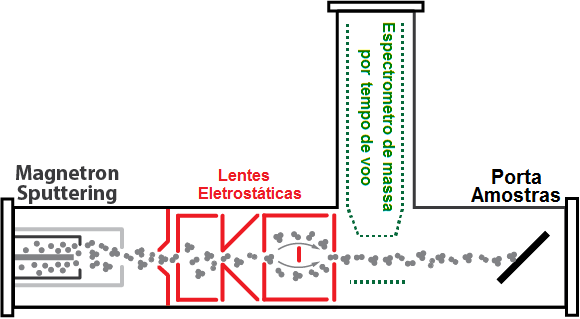
\includegraphics[width=0.8\textwidth]{images/foca/esquematico_foca_pt}
  \caption{ Diagrama da fonte de Fonte de \textit{Clusters} e Agregados. ``\textit{Magnetron Sputtering}'' é a fonte de átomos que se encontra dentro da câmara de agregação. Depois de produzido e agregado, o feixe passa por um conjunto de lentes eletrostáticas. Uma parte do feixe é desviado para o ``\textit{Espectrometro de massa por tempo de voo}'' (ToF), onde é realizada a aquisição do espectro de voo, outra parte é depositada na amostra - Adaptado\cite{livro_vitor}.  }
  \label{fig:esquema_foca}
\end{figure}

\begin{figure}
  \centering
  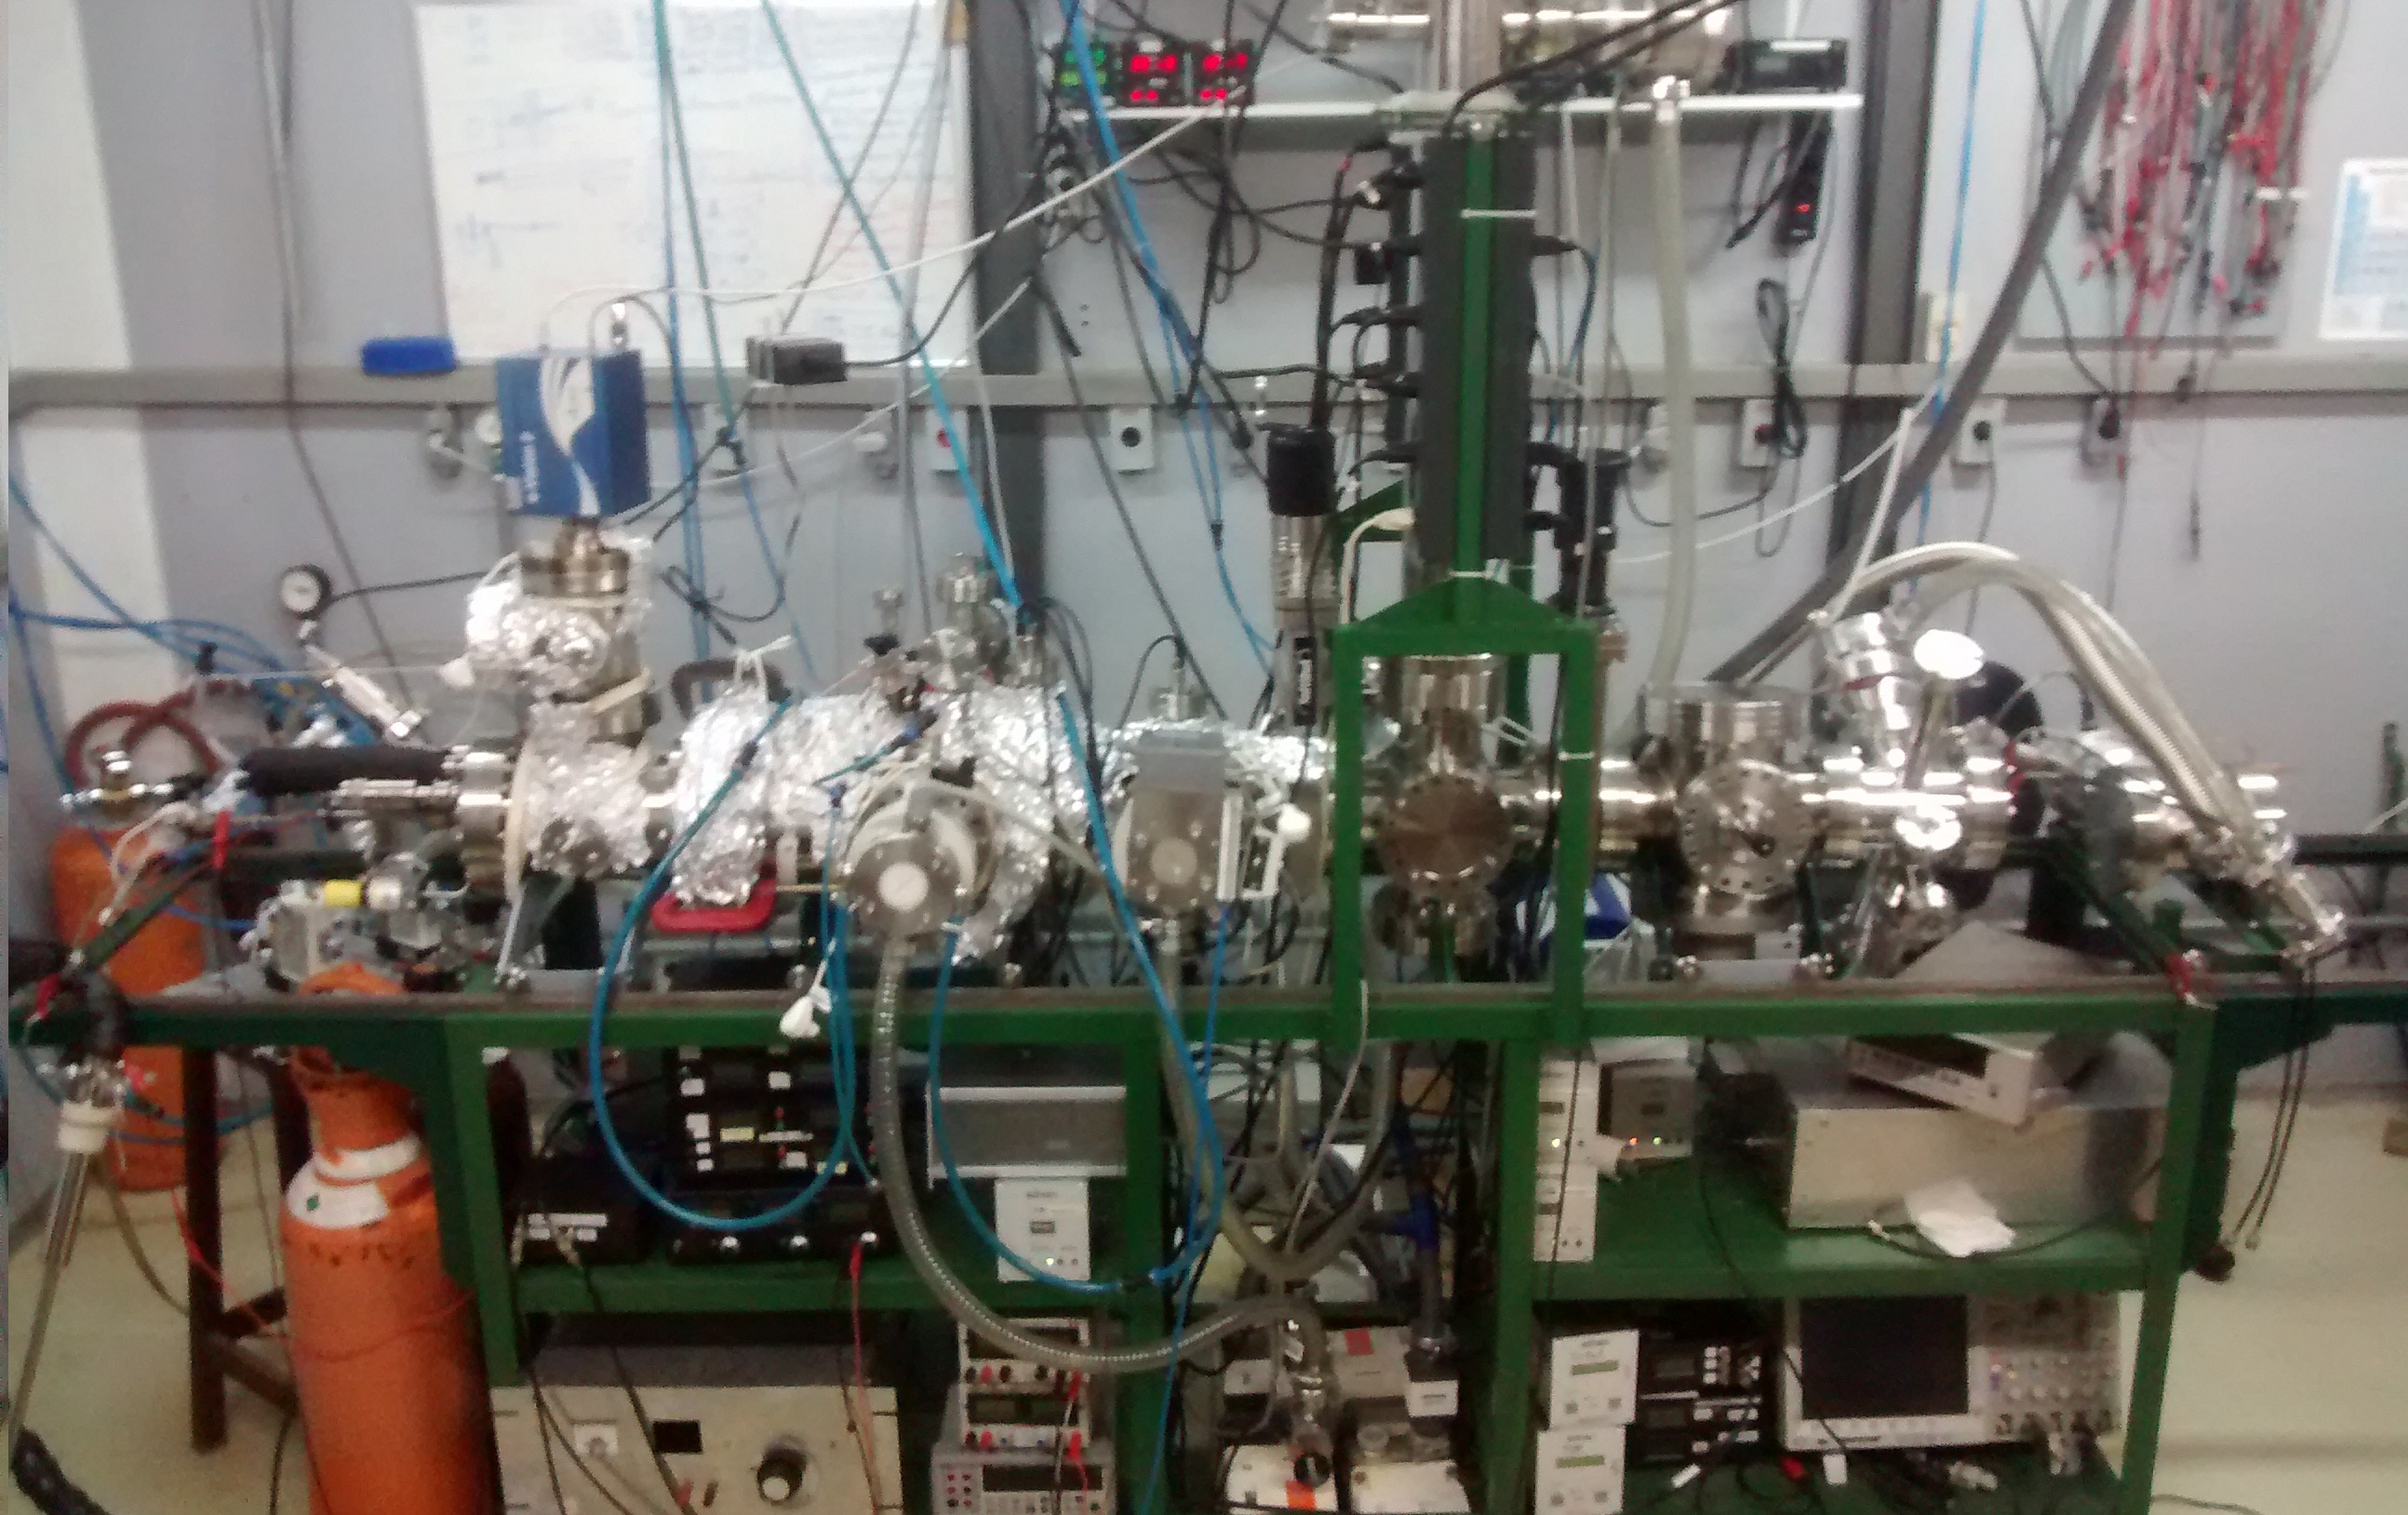
\includegraphics[width=0.7\textwidth]{images/foca/foto_foca}
  \caption{ Imagem real da  Fonte de \textit{Clusters} e Agregados.  }
  \label{fig:foto_foca}
\end{figure}



As lentes eletrostáticas citadas possuem as funções de: focalizar o feixe de íons, retirar as partículas neutras e, de acordo com o potencial aplicado nas lentes podem também funcionar como um filtro em função das energias das partículas. As lentes consistem em uma série de eletrodos de simetria cilíndrica nas quais são aplicadas potenciais. Uma foto das lentes pode ser vista na Figura \ref{fig:foto_lentes}. \textcolor{red}{As palavras skimmer, einzel e bessel não dizem para para o leitor.}

\textcolor{blue}{Com o intuito de colimar e amenizar efeitos de turbulências em grandes na a mistura de gás é utilizado o \textit{Skimmer}. O papel de focalizar o feixe é desenvolvido pelas lentes \textit{Einzel}. As lentes \textit{Bessel-Entrance} e \textit{Bessel-Box} retiram as partículas neutras presentes no feixe e também
atua como filtro de energia para as partículas carregadas.} 

\begin{figure}
  \centering
  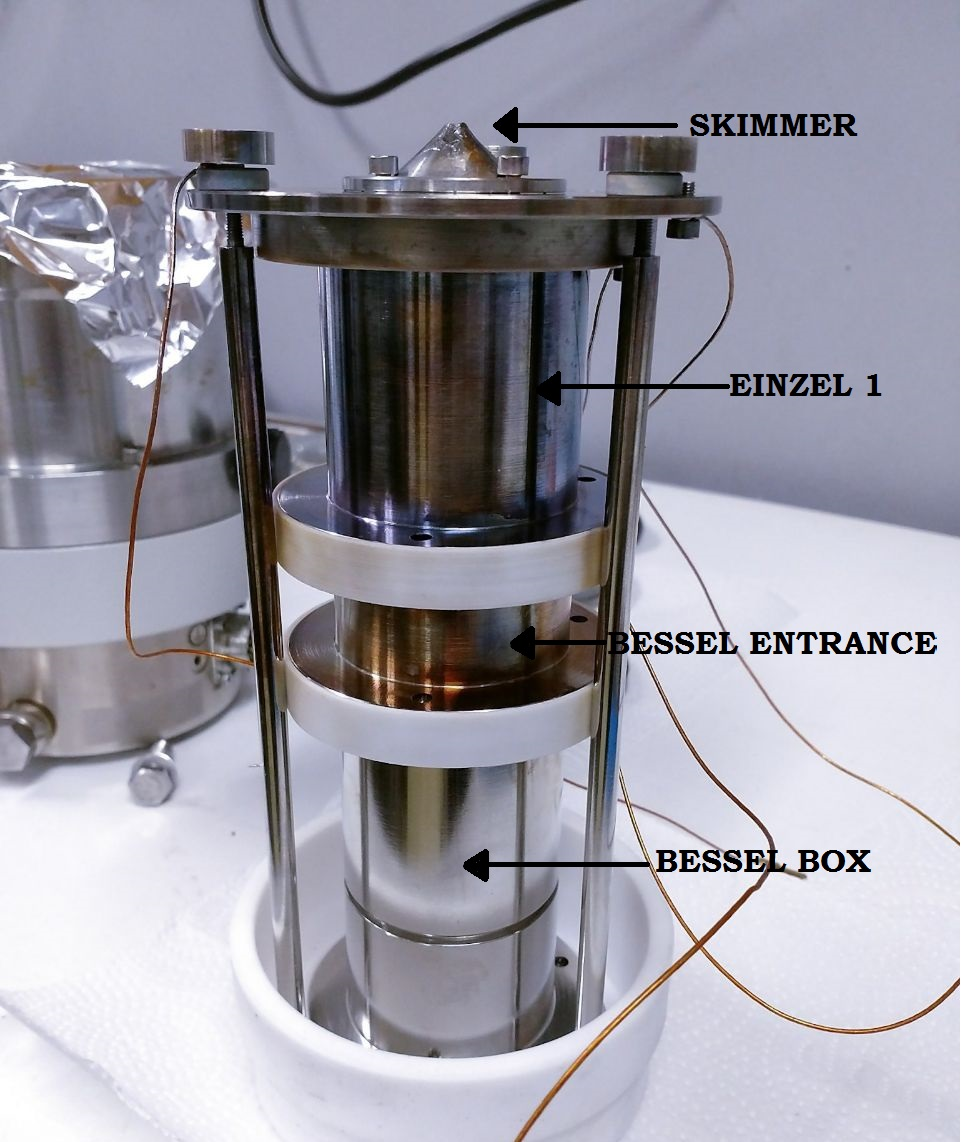
\includegraphics[width=0.6\textwidth]{images/foca/lentes}
  \caption{ Foto da lentes eletrostáticas.  }
  \label{fig:foto_lentes}
\end{figure}


Para gerar a nuvem de átomos, a FoCA utiliza um \textit{magnetron cilíndrico} \cite{ref_artigo_foca}, que caracteriza a produção desses \textit{clusters} por \textit{sputtering}. Aqui o alvo material que dará origem às nanopartículas possui o formato de um fio e fica localizado no eixo do \textit{magnetron}. A versatilidade dessa técnica encontra-se no fato que o alvo é multivalente, podendo ser composto de vários metais, incluindo ligas, como, por exemplo, a mistura ouro e prata, bastando entrelaçar os fios do metal de desejo para isso. Na Figura \ref{fig:magnetron}, podemos ver o plasma gerado no \textit{magnetron cilíndrico}. Pela presença de um campo elétrico, os íons são acelerados em direção ao alvo do metal de interesse e o erodem. Na Figura \ref{fig:alvo} é possível observar um alvo de prata, composto por um único fio, novo e ao lado um já erodido.

\begin{figure}
  \centering
  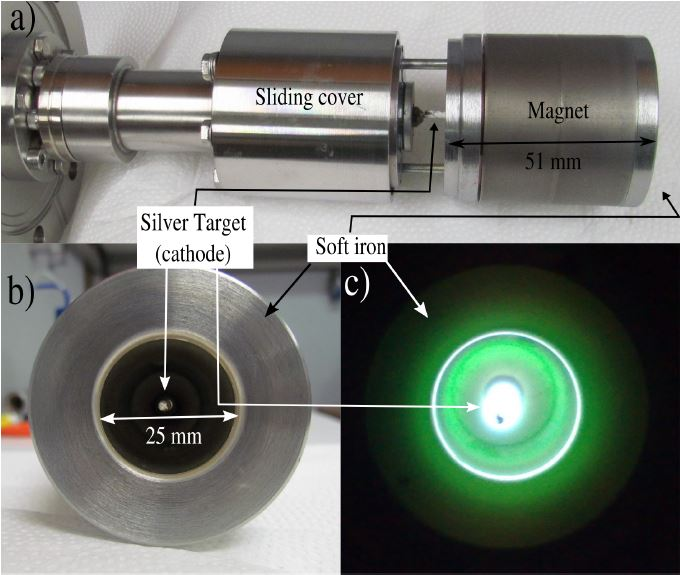
\includegraphics[width=0.75\textwidth]{images/foca/magnetron_cil}
  \caption{ (a) Magnetron cilíndrico oco caseiro com a tampa deslizante retraída para mostrar o alvo de prata. (b) vista frontal. (c) Vista frontal com plasma aberto. Observe a cor esverdeada ao redor do alvo, tipicamente vista na formação de plasma prateado.\cite{livro_vitor} }
  \label{fig:magnetron}  
\end{figure}



\begin{figure}
  \centering
  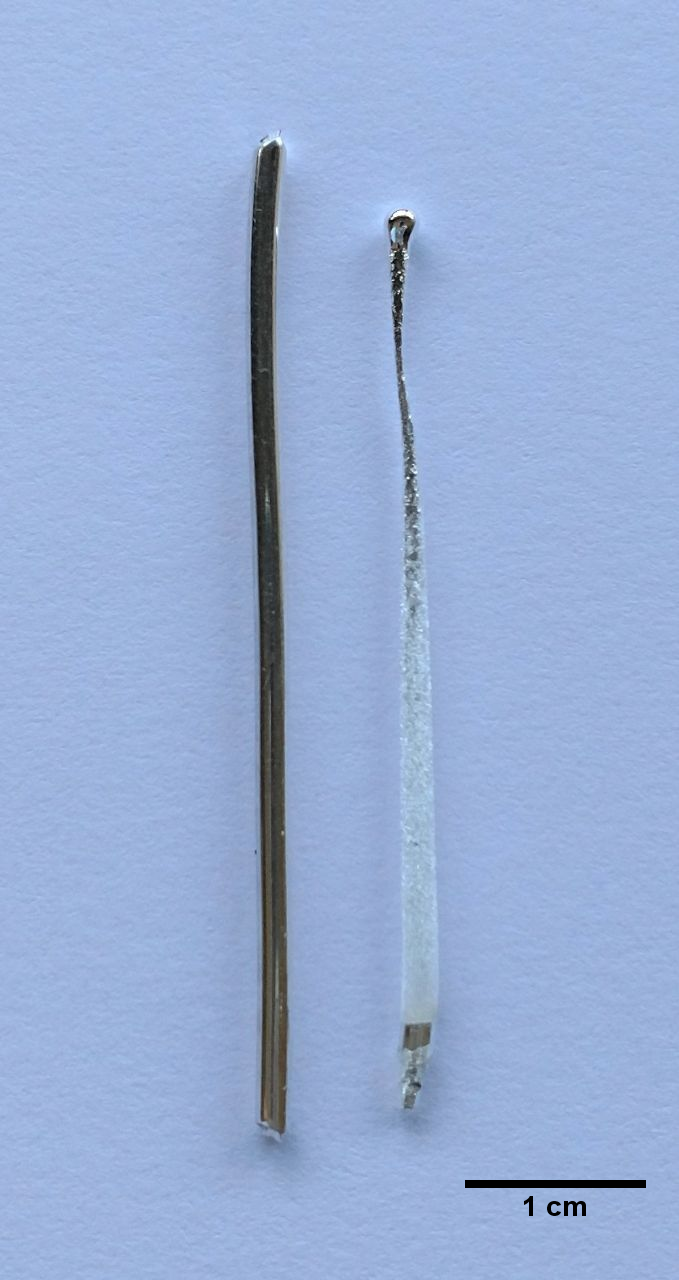
\includegraphics[width=0.3\textwidth]{images/foca/alvo}
  \caption{ Foto de um alvo de prata de fio único. À esquerda temos um alvo novo e à direita temos um alvo já corroído.  }
  \label{fig:alvo}
\end{figure}


%%%%%%%%%%%%%%_TOF_%%%%%%%%%%%%%%%%
\section{Espectrômetro de massa por tempo de voo}
\label{sec:tof}
Esta seção será dedicada a descrever o princípio de funcionamento da técnica de \textit{Time-of-flight Mass Spectrometers} (TOFMSs).
Pode-se observar o esquema do espectrômetro na Figura \ref{fig:tof}, onde o pulso elétrico fornece velocidade perpendicular ao feixe de partículas carregadas, que então viajam dentro de um tubo de voo - livre de variação de potencial elétrico - até encontrarem um detetor de corrente. Por sua vez, o detetor faz a contagem de íons em função dos tempos de chegada.

O TOFMSs funciona  baseado no fato de que, ao receber a mesma quantidade de energia fornecida por um campo elétrico pulsado, partículas com massas/carga diferentes adquirem velocidades distintas \cite{dissertacao_kevin}. Assim, as partículas mais leves atingirão o detector antes das partículas mais pesadas.

\begin{figure}
  \centering
  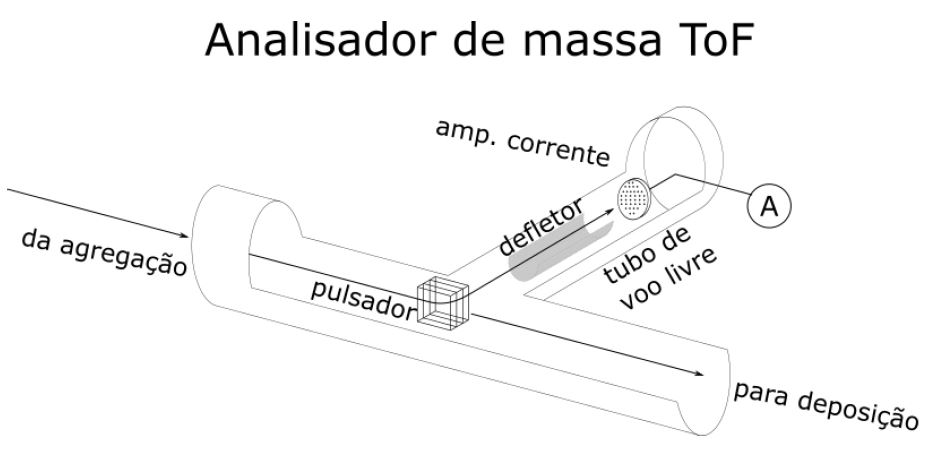
\includegraphics[width=1\textwidth]{images/foca/tof}
  \caption{ O pulsador é um conjunto de placas com campo pulsado, que confere uma velocidade perpendicular ao feixe de partículas eletricamente carregadas. Os defletores impedem que as partículas colidam com as paredes do tubo de voo livre. ``\textit{A}'' representa o detector de corrente, cuja função é realizar a contagem dos íons em função do tempo de chegada.  \cite{dissertacao_kevin}.  }
  \label{fig:tof}
\end{figure}

Para calcular o tempo de voo, vamos considerar um \textit{cluster} de massa $m$ e carga $q$. O campo elétrico vai fornecer energia cinética ($K = qV$) para a partícula, em que $V$ é a voltagem fornecida pelo pulsador. Assim, é possível expressar a velocidade da partícula como:

\begin{equation}
v = \sqrt[]{\frac{2qV}{m}}
\end{equation}

O detector de corrente está situado a uma distância $L$ da região onde a partícula adquire velocidade. Note que essa partícula levará um tempo $t_{voo}$ para atingir o detector, e esse tempo pode ser calculado por:

\begin{equation}
\label{eq:tempo_voo}
t_{voo} = L \cdot \sqrt[]{\frac{1}{2V}}  \sqrt[]{\frac{m}{q}} 
\end{equation}


A corrente que chega ao detector é convertida em tensão por um amplificador IV, e o sinal é exibido em um osciloscópio e, então, para aquisição dos dados utiliza-se um programa desenvolvido pelo grupo.

A variável $L$ possui o valor de um metro, o potencial aplicado é de $V = 7 $  kV, e o tempo de voo das partículas é fornecido pelo osciloscópio, possibilitando calcular a massa das partículas.

Note que utilizando a Equação \ref{eq:tempo_voo} é possível também calcular o $t_{voo}$ de uma partícula se soubermos a massa. Vamos fazer uma análise para o caso de um átomo de prata. Segundo a tabela periódica, um átomo de prata possui uma massa de $107,87$ unidades de massa atômica e convertendo sua massa para quilos, temos $1,79\times 10^{-25}$ kg. A carga de partícula é a carga elementar de um elétron $1,60\times 10^{-19}$ C, e então seu tempo de voo vai ser aproximadamente$17,6$ $\mu$s.

Podemos também escrever a massa de uma nanopartícula em função da massa de uma outra partícula da qual conhecemos a massa e o tempo de voo.

\begin{equation}
\label{eq:relacao_massa_tempo}
M = \left(\frac{t}{t'}\right)^2 \cdot M'
\end{equation}


É possível estabelecer uma relação que futuramente vai permitir diferenciar outros picos de prata, e então calibrar o espectro de partículas produzido, confirmando o que foi depositado na amostra.


A grande vantagem desse tipo de técnica, espectrometria de massa por tempo de voo, é que a obtenção da distribuição de tamanhos das nanopartículas produzidas é exibida em tempo real, assim qualquer variação indesejável no espectro é passível de correção, ainda durante o processo de deposição, por meio de ajuste  dos parâmetros da máquina. 


%%%%%%%%%%%%%%_LED_%%%%%%%%%%%%%%%%%
\section{Experimentos com luz ultravioleta}
\label{sec:led}

Nesta seção descreveremos o processo utilizado para iluminação dos \textit{Clusters} com luz ultravioleta.

\textcolor{red}{Precisa dizer qual o papel da luz ultra-violeta primeiro. Não lembro de te visto escrito no texto ainda.}

\textcolor{blue}{A incidência de luz ultravioleta sob o feixe de nanopartículas fornece energia para o mesmo. Desta forma um número maior de \textit{clusters} presentes no feixe poderão apresentar um maior grau de ionização; por consequência maior corrente e também um aparecimento mais frequênte de \textit{clusters} com \textit{"números mágicos"}.}

Para realizar experimentos com incidência de luz ultra violeta foi preciso montar um sistema de iluminação, que consiste em inserir um LED do UV, modelo \textit{UVTOP240 TO39} produzido pela \textit{Roithner Lasertechnik GmbH}, na fonte de agregados. Para isto foi instalado um passante de tensão para que o LED fique em dentro da máquina. Além disso, um sistema de alimentação com controle de corrente foi montado utilizando uma fonte de tensão.

O LED é baseado em AlGaN (Alumínio, Gálio e Nitrogênio), com um pico típico de comprimento de onda de $245 nm$ e potência de saída óptica de $30-70 \mu W$. Seu encapsulamento é metálico e hermeticamente fechado, com configuração de lente de vidro plano. Uma foto desse diodo pode ser vista na Figura \ref{fig:foto_led}.

\begin{figure}
  \centering
  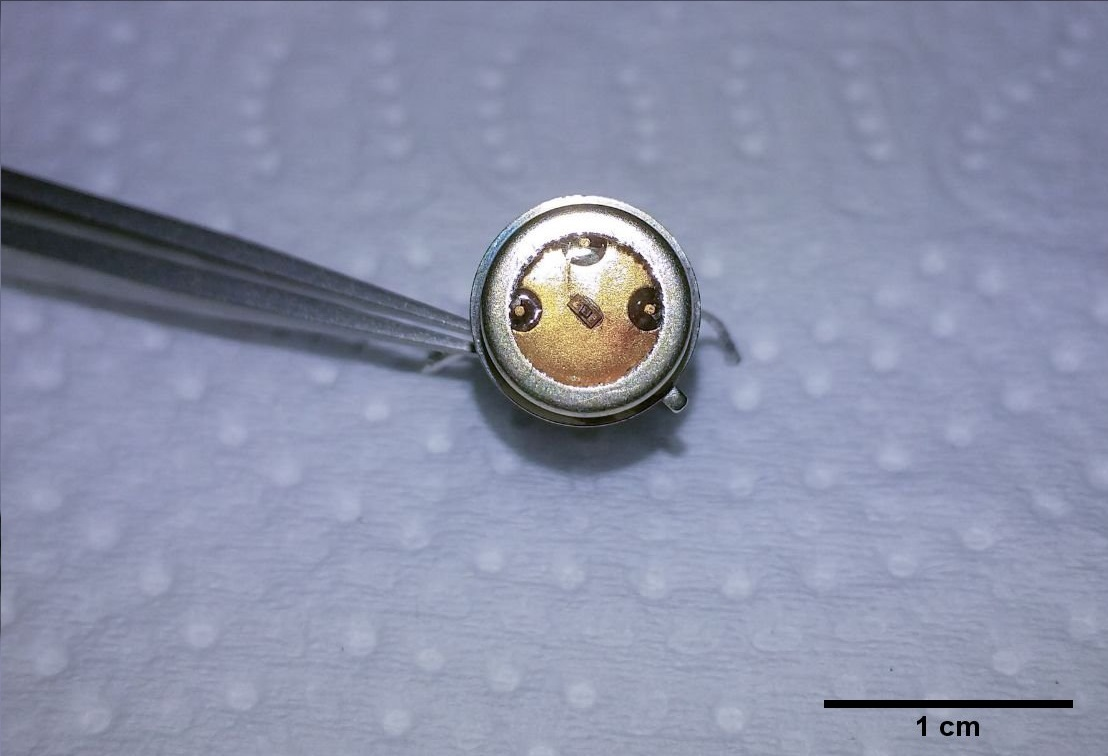
\includegraphics[width=0.7\textwidth]{images/foca/led_scale}
  \caption{ Foto do LED do UV, modelo UVTOP240 TO39, utilizado para ionização das nanopartículas.  }
  \label{fig:foto_led}
\end{figure}


Foi escolhido posicionar o LED entre a saída da câmara de agregação e a primeira lente eletrostática, como podemos ver na Figura \ref{fig:led_montagem}. Os testes do aparato consistem na aquisição da corrente de agregados produzidos e do seu espectro de massa sem o uso do LED e, posteriormente, com o LED. Com isso foi avaliado o possível aumento de ionização, como a incidência de luz afeta o espectro de massa do sistema de agregação e possíveis ajustes nos valores da tensões das lentes eletrostáticas.
Assim, foram realizados experimentos com incidência de luz ultra violeta (UV), induzindo a sua ionização, e foram comparados os espectros de abundância obtidos com e sem o uso da luz UV. 



\begin{figure}
  \centering
  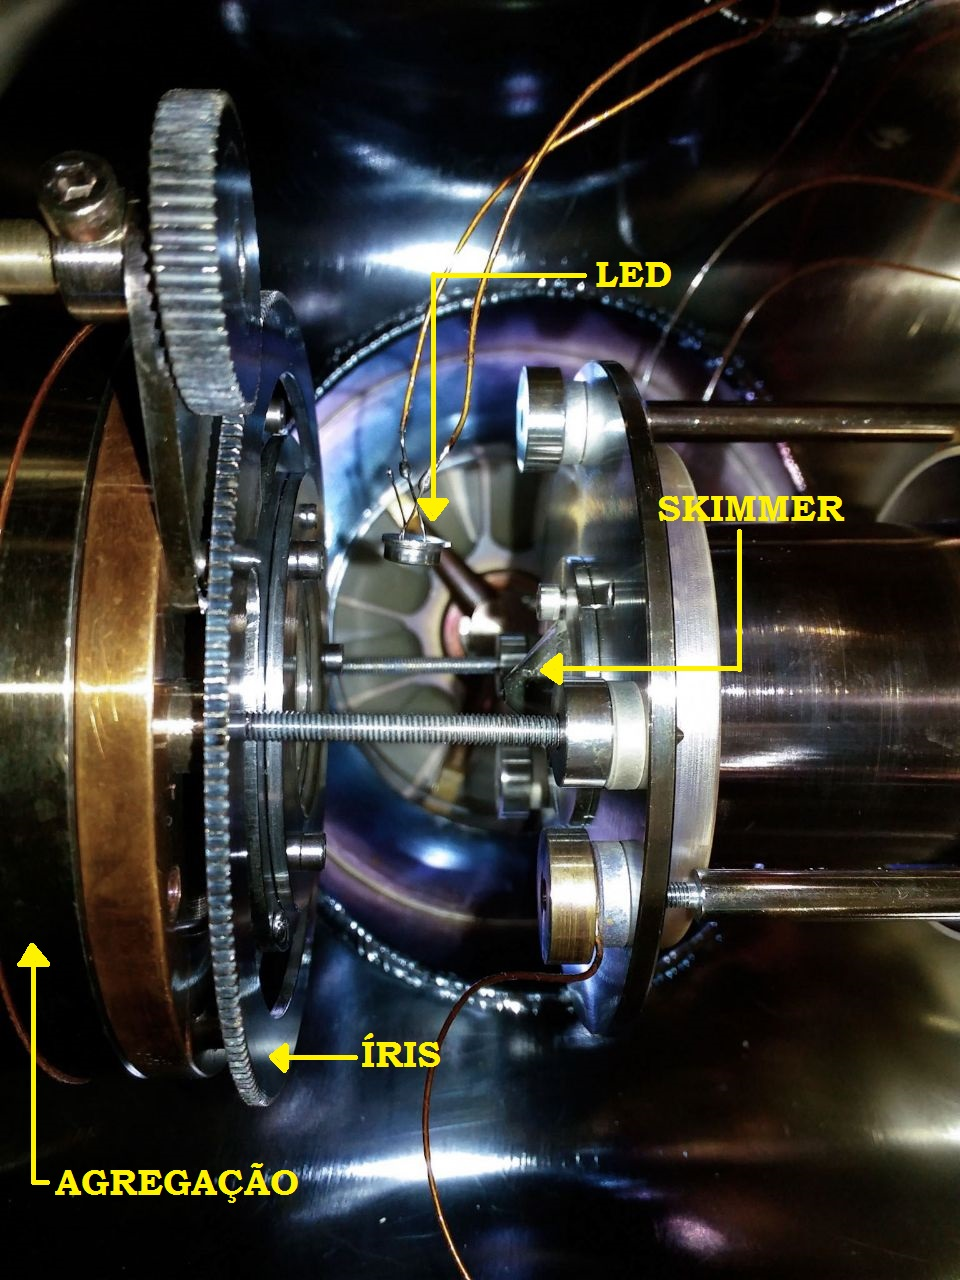
\includegraphics[width=0.5\textwidth]{images/foca/led_montagem}
  \caption{Foto do posicionamento do LED, localizado entre a câmara de deposição e a primeira lente eletrostática, Skimmer. Também está indicado a íris, peça que controla a pressão na câmara de agregação.}
  \label{fig:led_montagem}
\end{figure}



\chapter{Resultados}
\label{resultados}

Neste capítulo apresentaremos os espectros de massa referentes aos \textit{clusters} de prata, que caracterizam os resultados experimentais obtidos neste trabalho.

\section{Espectros de nanopartículas de prata}
\label{sec:result_producao_cluster}
Foram realizados quatro experimentos para obtenção dos espectros de prata. Para cada um foram obtidos os dados dos \textit{clusters} com e sem a incidência de luz ultra violeta. 

Os dados fornecidos pelo sistema de aquisição
fornece o tempo de voo das partículas e as intensidade dos picos, como pode ser visto na Figura \ref{fig:ex_dados_brutos}. Depois de adquirido, os dados são tratados de forma a minimizar os ruídos existentes, e é feita uma normalização pela eficiência do detector de corrente, uma vez que as partículas com menor massa são melhor detectadas do que as partículas de maiores massas. O mesmo espectro com o tratamento de dados realizado pode ser visto na Figura \ref{fig:0105_ledoff_dados_tratados}.




\begin{figure}
  \centering  
  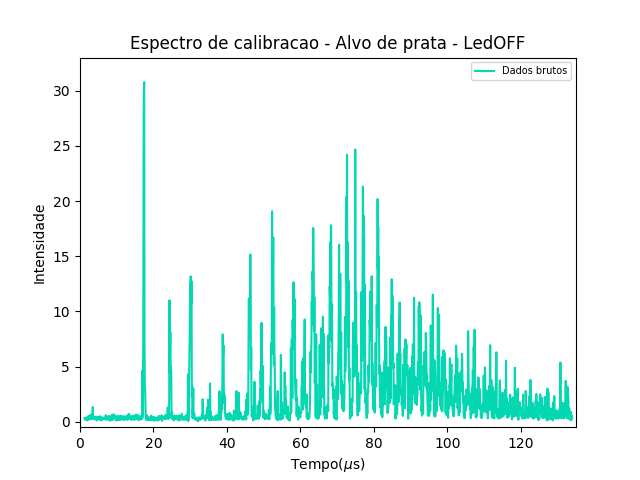
\includegraphics[width=0.7\textwidth]{exp_01/LedOFF_sem_tratamento.png}
  \caption{Espectro de calibração sem tratamento de dados.}
  \label{fig:ex_dados_brutos} 
\end{figure}

\begin{figure}
  \centering  
  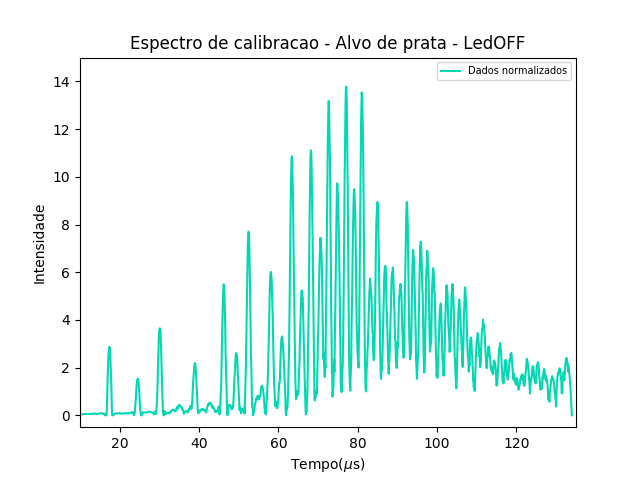
\includegraphics[width=0.7\textwidth]{exp_01/LedOFF_normalizado_mcp.png}
  \caption{Espectro de calibração com tratamento de dados.}
  \label{fig:0105_ledoff_dados_tratados} 
\end{figure}

Para indicar quais são os picos presentes nos espectros, e assim encontrar as indicações do número de prata ($Ag_{1},Ag_{2},Ag_{3}...$), é necessário realizar uma calibração, \textcolor{blue}{onde são relacionadas o tempo de voo de cada partícula com o quociente massas/carga, como explicitado na Equação \ref{eq:tempo_voo}}, de forma a obter uma tendência quadrática, como veremos a seguir.

Com o objetivo de obter uma maior precisão na determinação dos tempos de voo das partículas de prata, é traçado uma curva gaussiana em cima de cada pico do espectro. \textcolor{blue}{A gaussiana traçada possui uma largura de $2\mu$ segundos, fato esse que será utilizado para encontrar as incertezas dos dados obtidos.}

A Tabela \ref{tab:picos_encontados_01} mostra os valores dos picos encontrados, em comparação com os valores dos picos calculados teoricamente pela Equação \ref{eq:relacao_massa_tempo}. \textcolor{blue}{ Note que os resultados obtidos encontram-se dentro da margem de incerteza, implicando que os picos encontrados correspondem com os que eram esperados.} 

\begin{table}
\centering
\caption{I- Tempo de voo dos átomos de Prata}
\label{tab:picos_encontados_01}
\begin{tabular}{|c|c|c|c|c|c|c|}
\hline
\begin{tabular}[c]{@{}c@{}}Prata\\ (N)\end{tabular} & \begin{tabular}[c]{@{}c@{}}Massa\\ teórica\\ (u.m.a)\end{tabular} & \begin{tabular}[c]{@{}c@{}}LED OFF\\ Massa\\ calculada\\ $\pm \Delta m$\\ (u.m.a)\end{tabular} & \begin{tabular}[c]{@{}c@{}}LED ON\\ Massa\\ calculada\\ $\pm \Delta m$\\ (u.m.a)\end{tabular} & \begin{tabular}[c]{@{}c@{}}Tempo\\ teórico\\ ($\mu s$)\end{tabular} & \begin{tabular}[c]{@{}c@{}}LED OFF\\ Tempo\\ calculado\\ $\pm \Delta t$\\ ($\mu s$)\end{tabular} & \begin{tabular}[c]{@{}c@{}}LED ON\\ Tempo\\ calculado\\ $\pm \Delta t$\\ ($\mu s$)\end{tabular} \\ \hline 
1&107.86&104$\pm$25&106$\pm$26&17.30&17$\pm$2&17$\pm$2\\ \hline 
2&215.72&215$\pm$35&215$\pm$35&24.47&24$\pm$2&24$\pm$2\\ \hline 
3&323.58&322$\pm$42&324$\pm$42&29.96&30$\pm$2&30$\pm$2\\ \hline 
4&431.44&438$\pm$49&433$\pm$48&34.60&35$\pm$2&34$\pm$2\\ \hline 
5&539.30&536$\pm$54&538$\pm$54&38.68&38$\pm$2&38$\pm$2\\ \hline 
6&647.16&652$\pm$59&650$\pm$59&42.38&42$\pm$2&42$\pm$2\\ \hline 
7&755.02&756$\pm$64&756$\pm$63&45.77&46$\pm$2&46$\pm$2\\ \hline 
8&862.88&857$\pm$68&859$\pm$68&48.93&49$\pm$2&49$\pm$2\\ \hline 
9&970.74&966$\pm$72&968$\pm$72&51.90&52$\pm$2&52$\pm$2\\ \hline 
10&1078.60&1092$\pm$76&1087$\pm$76&54.71&55$\pm$2&55$\pm$2\\ \hline 
11&1186.46&1179$\pm$79&1180$\pm$79&57.38&58$\pm$2&58$\pm$2\\ \hline 
12&1294.32&1293$\pm$83&1291$\pm$83&59.93&60$\pm$2&60$\pm$2\\ \hline 
13&1402.18&1399$\pm$86&1400$\pm$86&62.38&63$\pm$2&63$\pm$2\\ \hline 
14&1510.04&1512$\pm$90&1509$\pm$89&64.73&65$\pm$2&65$\pm$2\\ \hline 
15&1617.90&1614$\pm$93&1618$\pm$92&67.00&68$\pm$2&68$\pm$2\\ \hline 
16&1725.76&1720$\pm$95&1728$\pm$95&69.20&70$\pm$2&70$\pm$2\\ \hline 
17&1833.62&1829$\pm$98&1833$\pm$98&71.33&72$\pm$2&72$\pm$2\\ \hline 
18&1941.48&1938$\pm$101&1941$\pm$101&73.40&74$\pm$2&74$\pm$2\\ \hline 
19&2049.34&2053$\pm$104&2048$\pm$104&75.41&77$\pm$2&76$\pm$2\\ \hline 
20&2157.20&2164$\pm$107&2158$\pm$107&77.37&79$\pm$2&79$\pm$2\\ \hline 
\end{tabular} 
\end{table} 


Sabendo o número de átomos de prata que corresponde a cada tempo de voo, é possível plotar uma curva de calibração, \textcolor{blue}{massa (em função da carga) $\times$ tempo}, e assim realizar uma ajuste de uma curva quadrática, onde os coeficientes que vão permitir identificar a massa de todo o espectro adquirido, seguindo a equação \ref{eq:0105_polinomio_calib_ledoff}. O ajuste do espectro em questão pode ser vista na Figura \ref{fig:1105_curva_calib_ledoff}.

\begin{equation}
\label{eq:0105_polinomio_calib_ledoff}
M(t) = 0,3304t^2 + 1,445t - 20,2
\end{equation}
\begin{figure}
  \centering  
  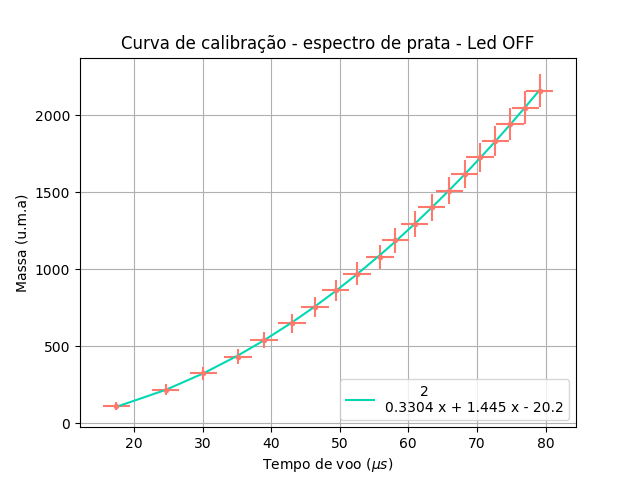
\includegraphics[width=0.7\textwidth]{exp_01/LEDOFF_curv+erro_calib.png}
  \caption{Curva de calibração.}
  \label{fig:1105_curva_calib_ledoff} 
\end{figure}



\textcolor{red}{Precisa explicar que é massa/carga}







Os erros foram calculados a partir da Equação \ref{eq:0105_polinomio_calib_ledoff}, da seguinte forma:

\begin{equation}
    \Delta M(t) = \frac{\partial M(t)}{\partial t} \times \Delta t
\end{equation}
onde $\Delta t = 2 \mu $ segundos.

E então para este caso, a equação para o cálculo do erro é dada por:

\begin{equation}
    \Delta M(t) = (2\times 0,3304 \times t + 1,445) \times 2
\end{equation}


Utilizando a Equação \ref{eq:0105_polinomio_calib_ledoff} é possível mudar o eixo de tempo de voo, da aquisição de dados, para o seu valor corresponde em massa, conforme do gráfico da Figura \ref{fig:0105_LEDOFF_espec_calib_ag_massa}.



\begin{figure}
  \centering  
  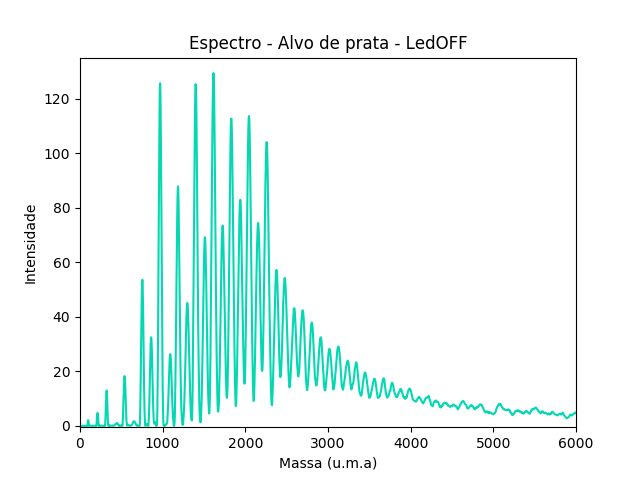
\includegraphics[width=0.7\textwidth]{graficos_resultados/0105_LEDOFF_espec_calib_ag_massa}
  \caption{Espectro de prata plotado na forma de intensidade por massa em unidade de massa atômica.}
  \label{fig:0105_LEDOFF_espec_calib_ag_massa} 
\end{figure}

Com o espectro em função da massa das \textit{clusters}, é possível identificar as partículas de prata com: um, dois, três... \textit{n} átomos, conforme mostra o gráfico da Figura \ref{fig:exp_01_LEDONOFF_N}. O gráfico apresenta também a relação entre os espectros com o LED ligado e desligado. Para obter a curva "\textit{LED ON}", foi utilizado o mesmo procedimento descrito anteriormente para a curva "\textit{LED OFF}".

Os espectros referentes ao dados com a incidência de luz ultra violeta, assim como a curva de calibração, serão apresentados no Apêndice \ref{sec:apendice}.

\begin{figure}
  \centering  
  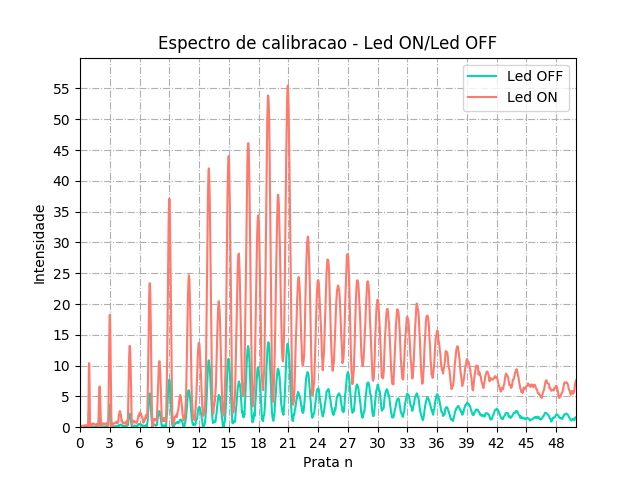
\includegraphics[width=0.7\textwidth]{exp_01/Led_ON_Led_OFF_espectro_calib_prata_N_}
  \caption{I-Espectro de prata, com LED ligado e desligado, na forma de intensidade por massa em unidade de massa atômica.}
  \label{fig:exp_01_LEDONOFF_N}
\end{figure}

Para obter uma boa estatística, foram realizados mais três experimentos os quais os espectro de prata, com LED ligado e desligado, na forma de intensidade por massa em unidade de massa atômica, podem ser vistos nas Figuras \ref{fig:exp_02_LEDONOFF_N}, \ref{fig:exp_03_LEDONOFF_N} e \ref{fig:exp_04_LEDONOFF_N}. As curvas de calibração, e as tabelas utilizadas para conversão serão apresentadas no Apêndice \ref{sec:apendice}.

\begin{figure}
  \centering  
  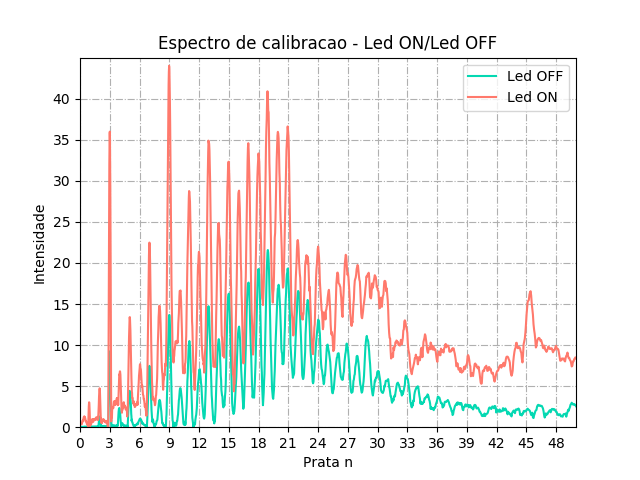
\includegraphics[width=0.7\textwidth]{exp_02/LED_ON_Led_OFF_espectro_calib_prata_N_.png}
  \caption{II- Espectro de prata, com LED ligado e desligado, na forma de intensidade por massa em unidade de massa atômica.}
  \label{fig:exp_02_LEDONOFF_N}
\end{figure}

\begin{figure}
  \centering  
  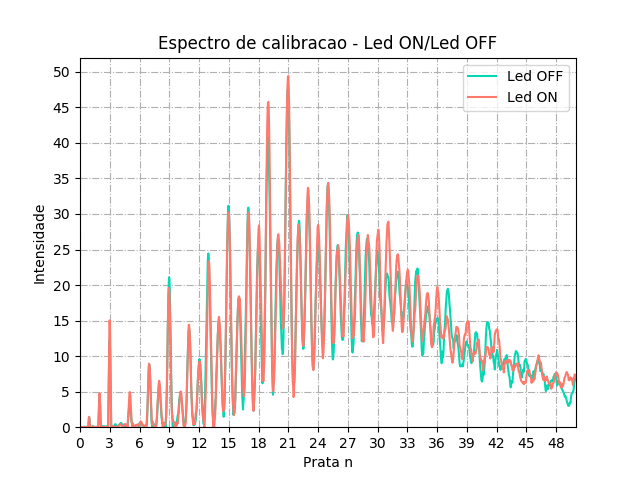
\includegraphics[width=0.7\textwidth]{exp_03/LED_ON_Led_OFF_espectro_calib_prata_N_.png}
  \caption{III-Espectro de prata, com LED ligado e desligado, na forma de intensidade por massa em unidade de massa atômica.}
  \label{fig:exp_03_LEDONOFF_N}
\end{figure}

\begin{figure}
  \centering  
  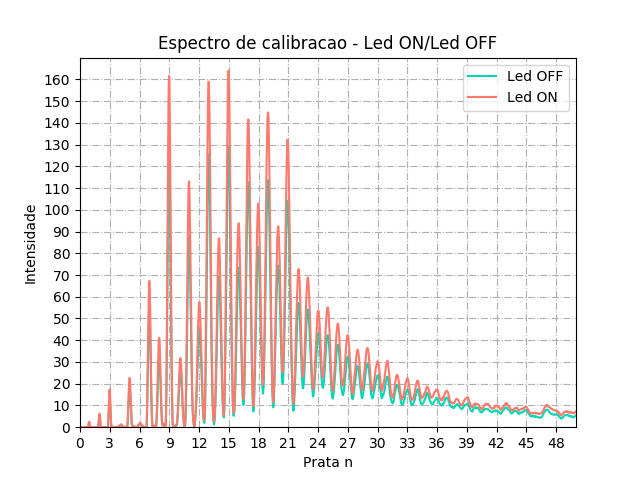
\includegraphics[width=0.7\textwidth]{exp_04/LED_ON_Led_OFF_espectro_calib_prata_N_.png}
  \caption{IV-Espectro de prata, com LED ligado e desligado, na forma de intensidade por massa em unidade de massa atômica.}
  \label{fig:exp_04_LEDONOFF_N}
\end{figure}

Note que nos resultados apresentados foi obtido o mesmo comportamento do experimento realizado por Katakuse et al \cite{KATAKUSE1985229}, em 1985 com, partícula de prata, já citado na secção \ref{sec:experimentos_teo}. Foram encontrados padrões com picos bem definidos em cada um espectro de massa e podemos apontar uma maior  abundância nos picos como número de átomos iguais, $n= 3,9,21,35...$. Esses picos ocorrem devido ao preenchimento das camadas eletrônicas, pelo princípio de exclusão de Pauli.

 No nosso caso as partículas de prata produzidas são carregada negativamente, ou seja, possuem um elétrons a mais, dessa forma temos que:
  \begin{equation*}
    Ag_{2} \to Ag_{2} + e^{-}
\end{equation*} 
 Fato esse que resulta nos "números mágicos" iguais à $n= 3,9,21,35...$. Além disso podemos notar que existe uma maior abundância dos \textit{clusters} com números ímpares de átomos em relação ao \textit{clusters} com números pares de átomos, isso também se deve a estabilidade dessas partículas.
 
 Fato que também podemos notar observando os espectros de partículas de prata apresentados nas Figuras \ref{fig:exp_01_LEDONOFF_N}, \ref{fig:exp_02_LEDONOFF_N} e \ref{fig:exp_04_LEDONOFF_N}, é que a intensidade dos picos, quando o LED encontra-se ligado, é superior a intensidade dos picos quando o LED encontra-se desligado. Isso ocorre devido ao fato da incidência de luz ultravioleta ioniza ainda mais as partículas que partem do \text{sputtering}, assim grande parte das partículas que antes eram neutras e eram barradas pelas lentes eletrostáticas agora são ionizadas e conseguem atingir a amostra, aumentando a intensidade da corrente medida.
 
 Os gráficos das Figuras \ref{fig:exp_01_picos_LEDONOFF_N}, \ref{fig:exp_02_picos_LEDONOFF_N} e \ref{fig:exp_04_picos_LEDONOFF_N} mostram mais explicitamente o fato citado.
 
 
 \begin{figure}
  \centering  
  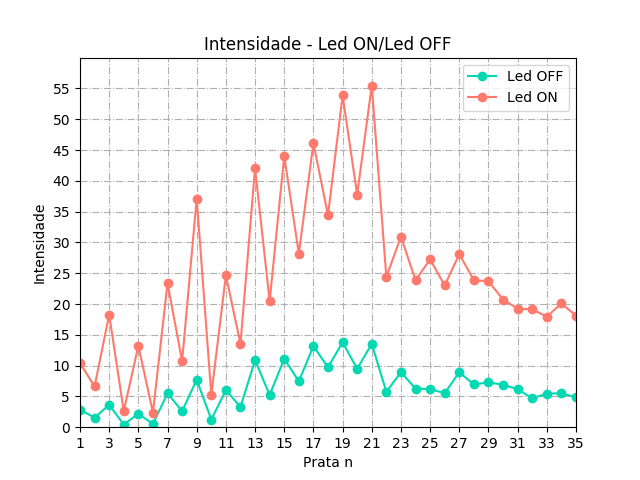
\includegraphics[width=0.7\textwidth]{exp_01/Led_ON_Led_OFF_intensidade_prata_N_.png}
  \caption{I - Relação de intensidade dos picos de prata, com LED ligado e desligado, na forma de intensidade por massa em unidade de massa atômica.}
  \label{fig:exp_01_picos_LEDONOFF_N}
\end{figure}
 
 \begin{figure}
  \centering  
  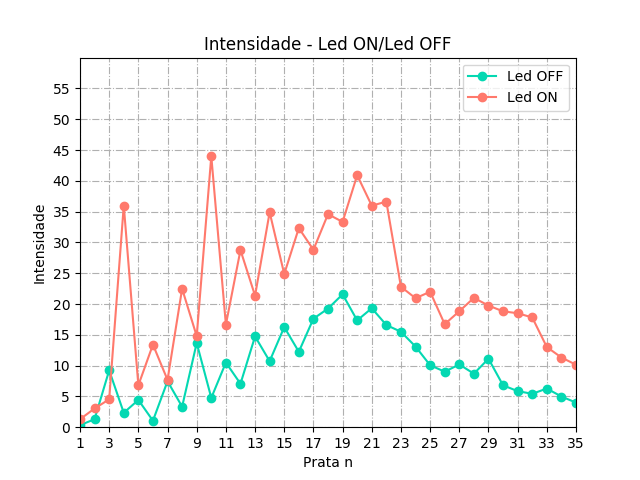
\includegraphics[width=0.7\textwidth]{exp_02/LED_ON_Led_OFF_intensidade_prata_N_.png}
  \caption{II - Relação de intensidade dos picos de prata, com LED ligado e desligado, na forma de intensidade por massa em unidade de massa atômica.}
  \label{fig:exp_02_picos_LEDONOFF_N}
\end{figure}
 
  \begin{figure}
  \centering  
  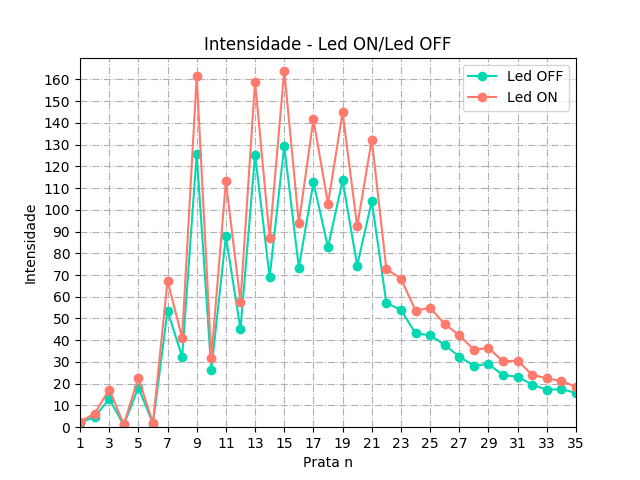
\includegraphics[width=0.7\textwidth]{exp_04/LED_ON_Led_OFF_intensidade_prata_N_.png}
  \caption{IV - Relação de intensidade dos picos de prata, com LED ligado e desligado, na forma de intensidade por massa em unidade de massa atômica.}
  \label{fig:exp_04_picos_LEDONOFF_N}
\end{figure}

Fato esse que não fica evidente no gráfico apresentado na Figura \ref{fig:exp_03_picos_LEDONOFF_N}, uma vez que esse experimento foi realizado no final do tempo de vida útil do alvo de prata e a corrente costuma cair rapidamente ao longo do tempo nesta situação. O protocolo experimental era realizar primeiro as medidas com o LED desligado e depois com o LED ligado, por isso temos alguns picos com o LED desligado que possuem maior intensidade. Com o alvo limitando a corrente fornecida, não havia um número átomos suficiente para ser ionizados pela luz ultravioleta e então não é possível notar uma grande diferença de intensidade.  

\begin{figure}
  \centering  
  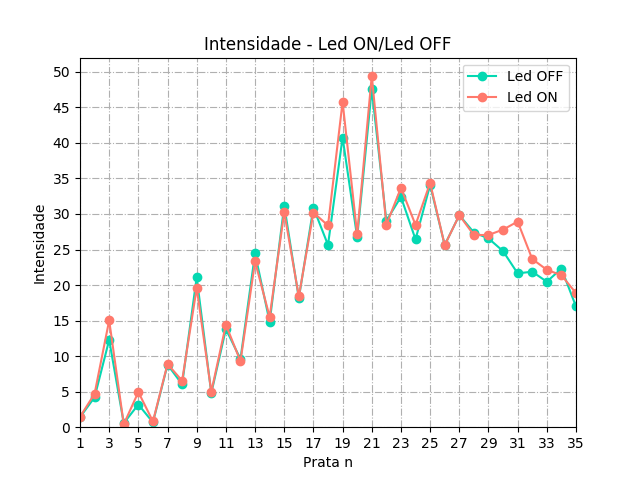
\includegraphics[width=0.7\textwidth]{exp_03/LED_ON_Led_OFF_intensidade_prata_N_.png}
  \caption{IV - Relação de intensidade dos picos de prata, com LED ligado e desligado, na forma de intensidade por massa em unidade de massa atômica.}
  \label{fig:exp_03_picos_LEDONOFF_N}
\end{figure}

\appendix
\chapter{Dados utilizados para calibração}
\label{sec:apendice}
Nesta secção serão apresentados os dados complementares utilizados para a calibração dos experimentos.

Para melhor organização os experimentos realizados serão divididos em: "Experimento I", "Experimento II", "Experimento III" e "Experimento IV".

\section{Experimento I}
A tabela e os dados utilizados para a calibração do espectro com LED desligado, já foram apresentadas na secção \ref{sec:result_producao_cluster}. A calibração do espectro com LED ligado pode ser vista na Figura \ref{fig:01_calib_ledON}.

\begin{figure}
  \centering  
  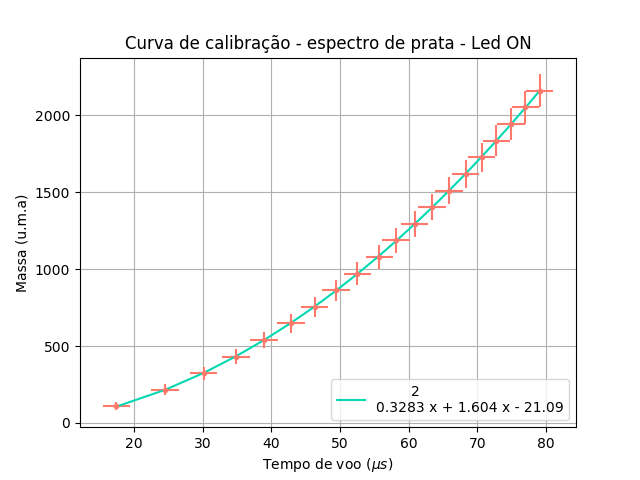
\includegraphics[width=0.7\textwidth]{exp_01/LEDON_curv+erro_calib.png}
  \caption{I- Curva de calibração para o LED ligado.}
  \label{fig:01_calib_ledON} 
\end{figure}

Utilizando o processamento de dados foi obtido o espectro de partículas em função do tempo e em função da massa, como pode ser visto respectivamente nas Figuras \ref{fig:01_ledon_dados_tratados} e \ref{fig:01_ledon_massa}.

\begin{figure}
  \centering  
  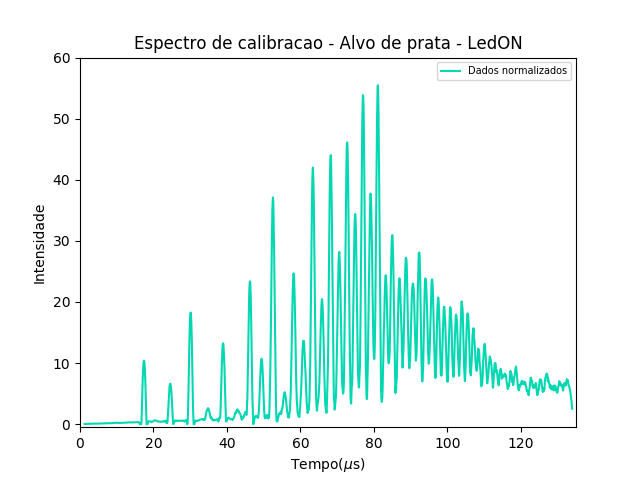
\includegraphics[width=0.7\textwidth]{exp_01/LedON_normalizado_mcp.png}
  \caption{I- Espectro de calibração com tratamento de dados.}
  \label{fig:01_ledon_dados_tratados} 
\end{figure}

\begin{figure}
  \centering  
  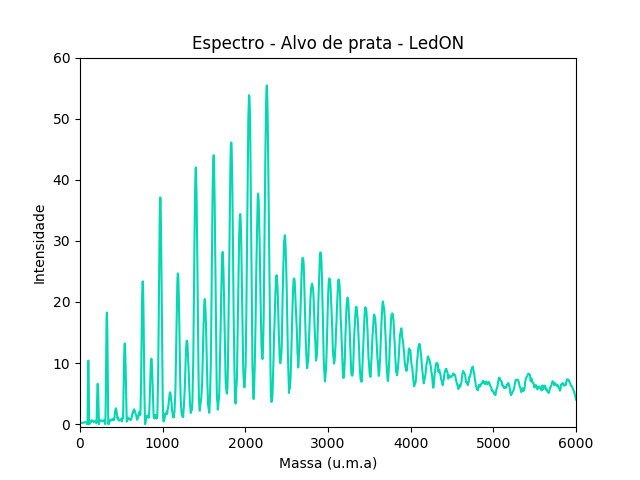
\includegraphics[width=0.7\textwidth]{exp_01/LEDON_espec_calib_ag_massa.png}
  \caption{I- Espectro de calibração com tratamento de dados.}
  \label{fig:01_ledon_massa} 
\end{figure}


\section{Experimento II}
A tabela e os dados utilizados para a calibração de ambos os estados do LED, pode ser vista na Tabela \ref{tab:picos_encontados_02}, assim como as curvas de calibração dos espectros que correspondem as Figuras \ref{fig:02_calib_ledOFF} e \ref{fig:02_calib_ledON}.

\begin{figure}
  \centering  
  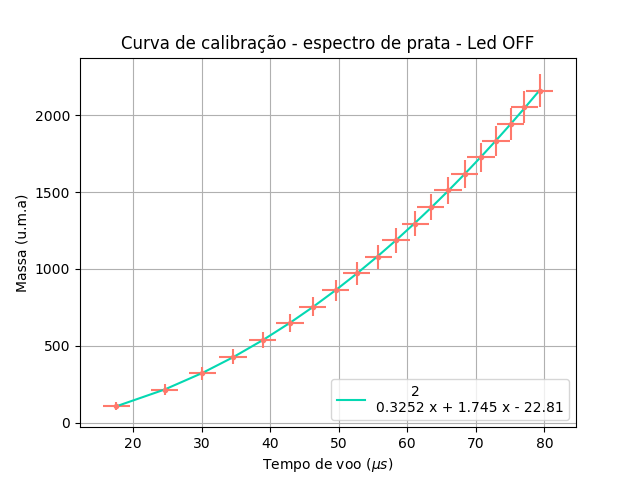
\includegraphics[width=0.7\textwidth]{exp_02/LEDOFF_curv+erro_calib.png}
  \caption{II- Curva de calibração para o LED ligado.}
  \label{fig:02_calib_ledOFF} 
\end{figure}

\begin{figure}
  \centering  
  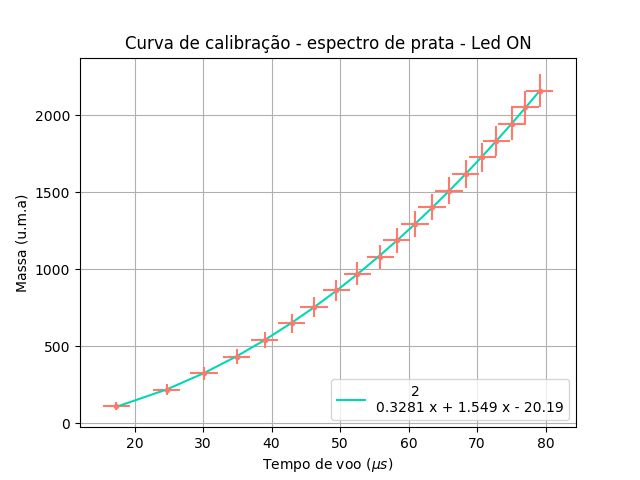
\includegraphics[width=0.7\textwidth]{exp_02/LEDON_curv+erro_calib.png}
  \caption{II- Curva de calibração para o LED ligado.}
  \label{fig:02_calib_ledON} 
\end{figure}

\begin{table}
\centering
\caption{Tempo de voo dos �tomos de Prata}
\label{tab:picos_encontados}
\begin{tabular}{|c|c|c|c|c|c|c|}
\hline
\begin{tabular}[c]{@{}c@{}}Prata\\ (N)\end{tabular} & \begin{tabular}[c]{@{}c@{}}Massa\\ te�rica\\ (u.m.a)\end{tabular} & \begin{tabular}[c]{@{}c@{}}LED OFF\\ Massa\\ calculada\\ $\pm \Delta m$\\ (u.m.a)\end{tabular} & \begin{tabular}[c]{@{}c@{}}LED ON\\ Massa\\ calculada\\ $\pm \Delta m$\\ (u.m.a)\end{tabular} & \begin{tabular}[c]{@{}c@{}}Tempo\\ te�rico\\ ($\mu s$)\end{tabular} & \begin{tabular}[c]{@{}c@{}}LED OFF\\ Tempo\\ calculado\\ $\pm \Delta t$\\ ($\mu s$)\end{tabular} & \begin{tabular}[c]{@{}c@{}}LED ON\\ Tempo\\ calculado\\ $\pm \Delta t$\\ ($\mu s$)\end{tabular} \\ \hline 
1&107.86&108$\pm$26&105$\pm$25&17.30&17$\pm$2&17$\pm$2\\ \hline 
2&215.72&216$\pm$35&217$\pm$35&24.47&24$\pm$2&24$\pm$2\\ \hline 
3&323.58&324$\pm$42&324$\pm$42&29.96&30$\pm$2&30$\pm$2\\ \hline 
4&431.44&426$\pm$48&433$\pm$48&34.60&34$\pm$2&34$\pm$2\\ \hline 
5&539.30&537$\pm$54&539$\pm$54&38.68&38$\pm$2&38$\pm$2\\ \hline 
6&647.16&651$\pm$59&650$\pm$59&42.38&42$\pm$2&42$\pm$2\\ \hline 
7&755.02&751$\pm$63&751$\pm$63&45.77&46$\pm$2&46$\pm$2\\ \hline 
8&862.88&862$\pm$67&859$\pm$68&48.93&49$\pm$2&49$\pm$2\\ \hline 
9&970.74&968$\pm$71&966$\pm$72&51.90&52$\pm$2&52$\pm$2\\ \hline 
10&1078.60&1087$\pm$76&1090$\pm$76&54.71&55$\pm$2&55$\pm$2\\ \hline 
11&1186.46&1186$\pm$79&1184$\pm$79&57.38&58$\pm$2&58$\pm$2\\ \hline 
12&1294.32&1300$\pm$83&1291$\pm$83&59.93&61$\pm$2&60$\pm$2\\ \hline 
13&1402.18&1395$\pm$85&1396$\pm$86&62.38&63$\pm$2&63$\pm$2\\ \hline 
14&1510.04&1507$\pm$89&1505$\pm$89&64.73&65$\pm$2&65$\pm$2\\ \hline 
15&1617.90&1616$\pm$92&1618$\pm$92&67.00&68$\pm$2&68$\pm$2\\ \hline 
16&1725.76&1728$\pm$95&1732$\pm$95&69.20&70$\pm$2&70$\pm$2\\ \hline 
17&1833.62&1833$\pm$98&1833$\pm$98&71.33&72$\pm$2&72$\pm$2\\ \hline 
18&1941.48&1941$\pm$101&1945$\pm$101&73.40&75$\pm$2&75$\pm$2\\ \hline 
19&2049.34&2043$\pm$103&2044$\pm$104&75.41&77$\pm$2&76$\pm$2\\ \hline 
20&2157.20&2161$\pm$106&2158$\pm$106&77.37&79$\pm$2&79$\pm$2\\ \hline 
\end{tabular} 
\end{table} 


Utilizando o processamento de dados foi obtido o espectro de partículas em função do tempo e em função da massa, como pode ser visto respectivamente nas Figuras \ref{fig:02_ledoff_dados_tratados}, \ref{fig:02_ledoff_massa}, \ref{fig:02_ledon_dados_tratados} e \ref{fig:02_ledon_massa}.

\begin{figure}
  \centering  
  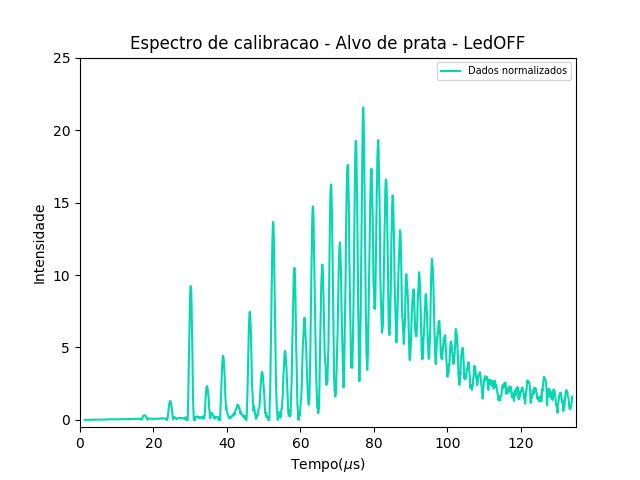
\includegraphics[width=0.7\textwidth]{exp_02/LEDOFF_normalizado_mcp.png}
  \caption{II- Espectro de calibração com tratamento de dados.}
  \label{fig:02_ledoff_dados_tratados} 
\end{figure}

\begin{figure}
  \centering  
  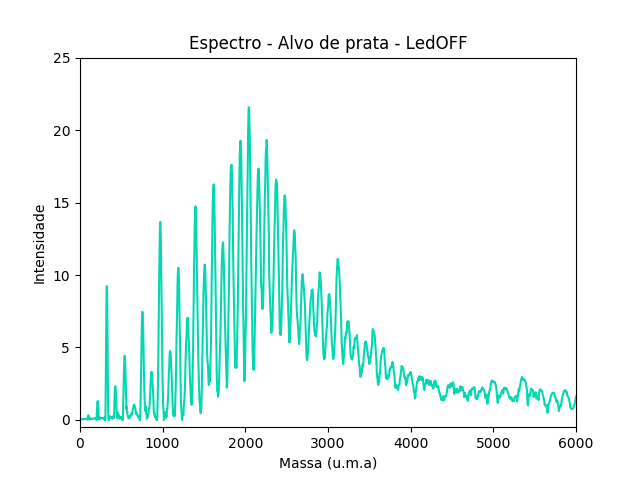
\includegraphics[width=0.7\textwidth]{exp_02/LEDOFF_espec_calib_ag_massa.png}
  \caption{II- Espectro de calibração com tratamento de dados.}
  \label{fig:02_ledoff_massa} 
\end{figure}



\begin{figure}
  \centering  
  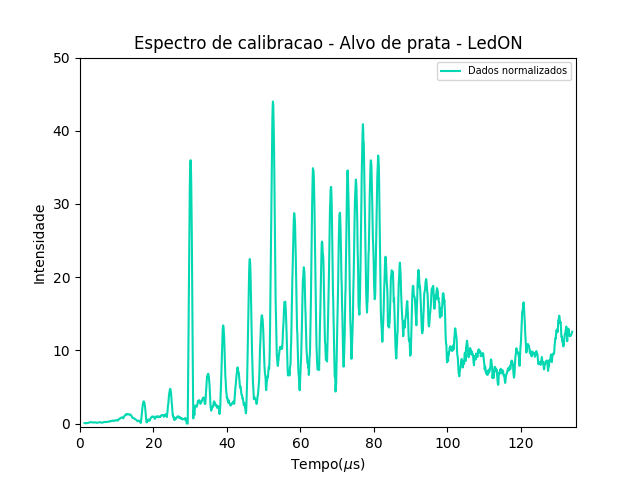
\includegraphics[width=0.7\textwidth]{exp_02/LEDON_normalizado_mcp.png}
  \caption{II- Espectro de calibração com tratamento de dados.}
  \label{fig:02_ledon_dados_tratados} 
\end{figure}

\begin{figure}
  \centering  
  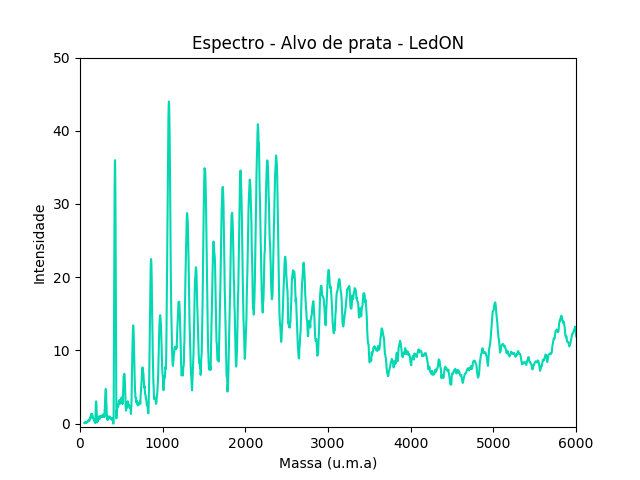
\includegraphics[width=0.7\textwidth]{exp_02/LEDON_espec_calib_ag_massa.png}
  \caption{II- Espectro de calibração com tratamento de dados.}
  \label{fig:02_ledon_massa} 
\end{figure}

\section{Experimento III}
A tabela e os dados utilizados para a calibração de ambos os estados do LED, pode ser vista na Tabela \ref{tab:picos_encontados_03}, assim como as curvas de calibração dos espectros que correspondem as Figuras \ref{fig:03_calib_ledOFF} e \ref{fig:03_calib_ledON}.

\begin{figure}
  \centering  
  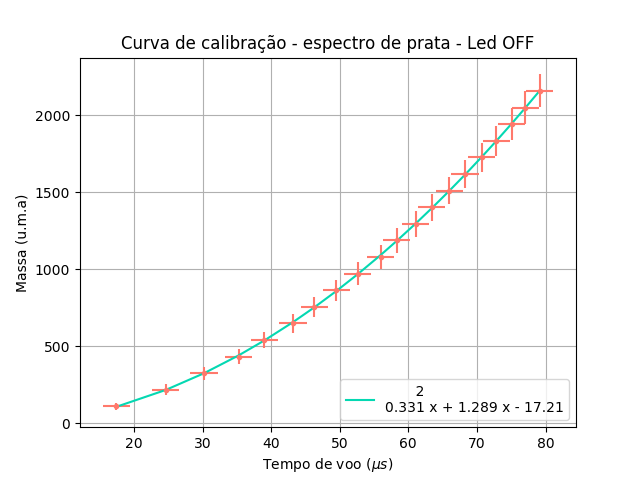
\includegraphics[width=0.7\textwidth]{exp_03/LEDOFF_curv+erro_calib.png}
  \caption{III- Curva de calibração para o LED ligado.}
  \label{fig:03_calib_ledOFF} 
\end{figure}

\begin{figure}
  \centering  
  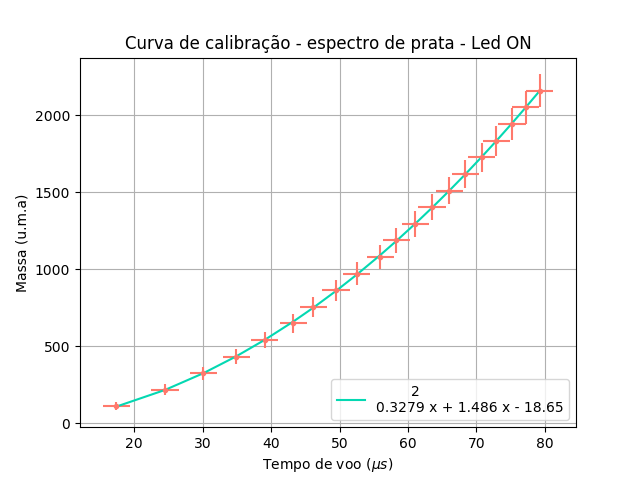
\includegraphics[width=0.7\textwidth]{exp_03/LEDON_curv+erro_calib.png}
  \caption{III- Curva de calibração para o LED ligado.}
  \label{fig:03_calib_ledON} 
\end{figure}

\begin{table}
\centering
\caption{Tempo de voo dos átomos de Prata}
\label{tab:picos_encontados_03}
\begin{tabular}{|c|c|c|c|c|c|c|}
\hline
\begin{tabular}[c]{@{}c@{}}Prata\\ (N)\end{tabular} & \begin{tabular}[c]{@{}c@{}}Massa\\ teórica\\ (u.m.a)\end{tabular} & \begin{tabular}[c]{@{}c@{}}LED OFF\\ Massa\\ calculada\\ $\pm \Delta m$\\ (u.m.a)\end{tabular} & \begin{tabular}[c]{@{}c@{}}LED ON\\ Massa\\ calculada\\ $\pm \Delta m$\\ (u.m.a)\end{tabular} & \begin{tabular}[c]{@{}c@{}}Tempo\\ teórico\\ ($\mu s$)\end{tabular} & \begin{tabular}[c]{@{}c@{}}LED OFF\\ Tempo\\ calculado\\ $\pm \Delta t$\\ ($\mu s$)\end{tabular} & \begin{tabular}[c]{@{}c@{}}LED ON\\ Tempo\\ calculado\\ $\pm \Delta t$\\ ($\mu s$)\end{tabular} \\ \hline 
1&107.86&105$\pm$25&106$\pm$25&17.30&17$\pm$2&17$\pm$2\\ \hline 
2&215.72&214$\pm$35&214$\pm$35&24.47&24$\pm$2&24$\pm$2\\ \hline 
3&323.58&323$\pm$42&323$\pm$42&29.96&30$\pm$2&30$\pm$2\\ \hline 
4&431.44&439$\pm$49&433$\pm$48&34.60&35$\pm$2&34$\pm$2\\ \hline 
5&539.30&536$\pm$54&540$\pm$54&38.68&38$\pm$2&39$\pm$2\\ \hline 
6&647.16&655$\pm$59&658$\pm$59&42.38&43$\pm$2&43$\pm$2\\ \hline 
7&755.02&751$\pm$63&749$\pm$63&45.77&46$\pm$2&46$\pm$2\\ \hline 
8&862.88&856$\pm$68&857$\pm$67&48.93&49$\pm$2&49$\pm$2\\ \hline 
9&970.74&966$\pm$72&963$\pm$71&51.90&52$\pm$2&52$\pm$2\\ \hline 
10&1078.60&1091$\pm$76&1091$\pm$76&54.71&55$\pm$2&55$\pm$2\\ \hline 
11&1186.46&1182$\pm$79&1181$\pm$79&57.38&58$\pm$2&58$\pm$2\\ \hline 
12&1294.32&1296$\pm$83&1295$\pm$83&59.93&61$\pm$2&61$\pm$2\\ \hline 
13&1402.18&1395$\pm$86&1396$\pm$86&62.38&63$\pm$2&63$\pm$2\\ \hline 
14&1510.04&1507$\pm$89&1509$\pm$89&64.73&65$\pm$2&66$\pm$2\\ \hline 
15&1617.90&1614$\pm$92&1615$\pm$92&67.00&68$\pm$2&68$\pm$2\\ \hline 
16&1725.76&1727$\pm$96&1728$\pm$95&69.20&70$\pm$2&70$\pm$2\\ \hline 
17&1833.62&1832$\pm$99&1833$\pm$98&71.33&72$\pm$2&72$\pm$2\\ \hline 
18&1941.48&1945$\pm$101&1945$\pm$101&73.40&75$\pm$2&75$\pm$2\\ \hline 
19&2049.34&2048$\pm$104&2048$\pm$104&75.41&77$\pm$2&77$\pm$2\\ \hline 
20&2157.20&2159$\pm$107&2157$\pm$106&77.37&79$\pm$2&79$\pm$2\\ \hline 
\end{tabular} 
\end{table} 


Utilizando o processamento de dados foi obtido o espectro de partículas em função do tempo e em função da massa, como pode ser visto respectivamente nas Figuras \ref{fig:03_ledoff_dados_tratados}, \ref{fig:03_ledoff_massa}, \ref{fig:03_ledon_dados_tratados} e \ref{fig:03_ledon_massa}.

\begin{figure}
  \centering  
  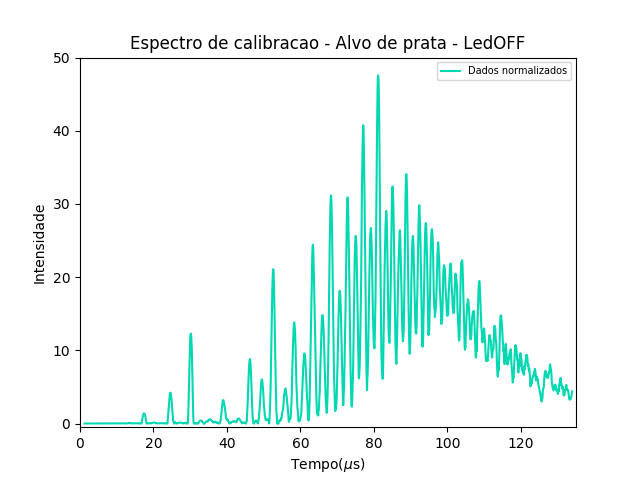
\includegraphics[width=0.7\textwidth]{exp_03/LEDOFF_normalizado_mcp.png}
  \caption{III- Espectro de calibração com tratamento de dados.}
  \label{fig:03_ledoff_dados_tratados} 
\end{figure}

\begin{figure}
  \centering  
  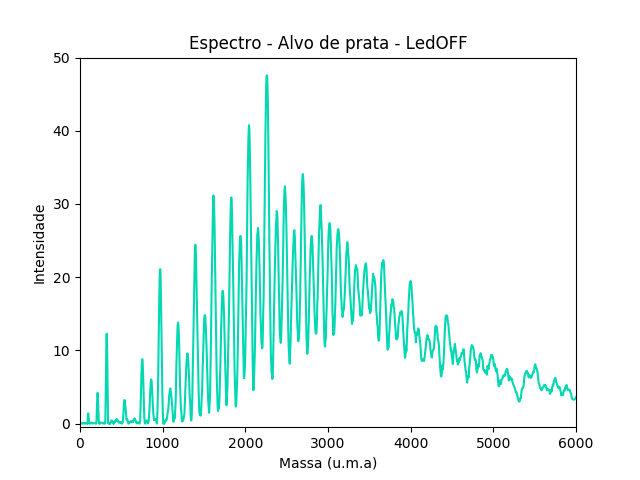
\includegraphics[width=0.7\textwidth]{exp_03/LEDOFF_espec_calib_ag_massa.png}
  \caption{III- Espectro de calibração com tratamento de dados.}
  \label{fig:03_ledoff_massa} 
\end{figure}



\begin{figure}
  \centering  
  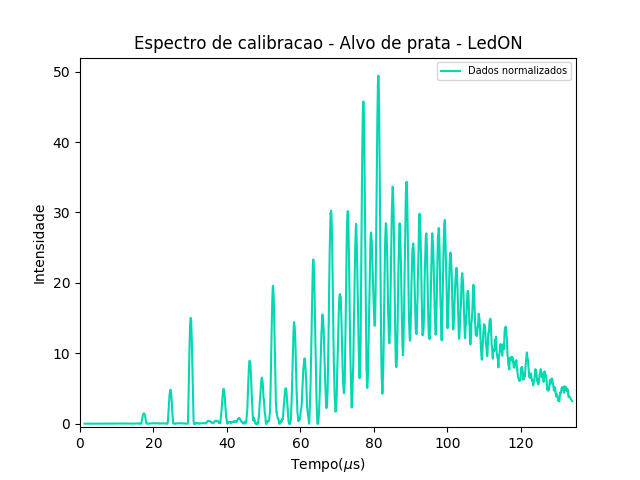
\includegraphics[width=0.7\textwidth]{exp_03/LEDON_normalizado_mcp.png}
  \caption{III- Espectro de calibração com tratamento de dados.}
  \label{fig:03_ledon_dados_tratados} 
\end{figure}

\begin{figure}
  \centering  
  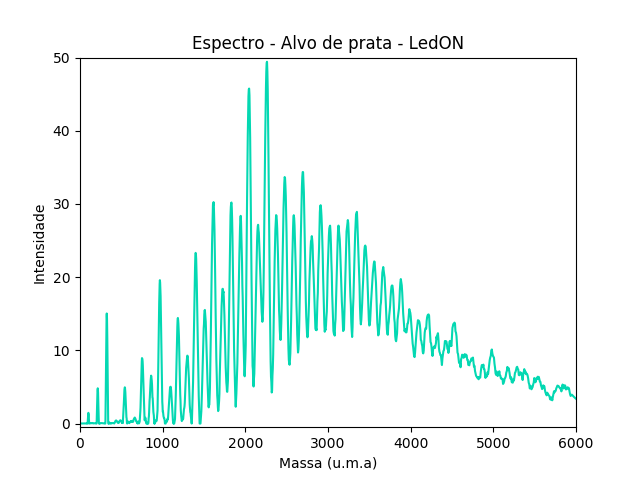
\includegraphics[width=0.7\textwidth]{exp_03/LEDON_espec_calib_ag_massa.png}
  \caption{III- Espectro de calibração com tratamento de dados.}
  \label{fig:03_ledon_massa} 
\end{figure}

\section{Experimento IV}
A tabela e os dados utilizados para a calibração de ambos os estados do LED, pode ser vista na Tabela \ref{tab:picos_encontados_04}, assim como as curvas de calibração dos espectros que correspondem as Figuras \ref{fig:04_calib_ledOFF} e \ref{fig:04_calib_ledON}.

\begin{figure}
  \centering  
  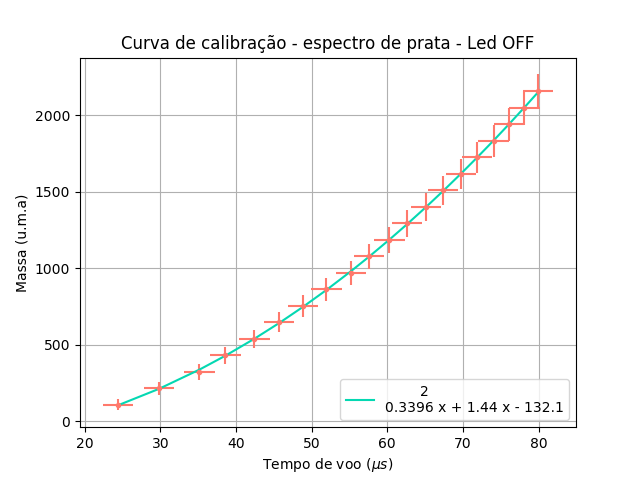
\includegraphics[width=0.7\textwidth]{exp_04/LEDOFF_curv+erro_calib.png}
  \caption{IV- Curva de calibração para o LED ligado.}
  \label{fig:04_calib_ledOFF} 
\end{figure}

\begin{figure}
  \centering  
  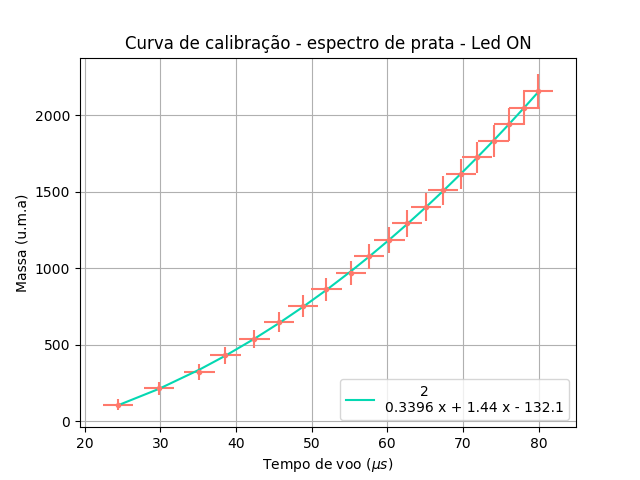
\includegraphics[width=0.7\textwidth]{exp_04/LEDON_curv+erro_calib.png}
  \caption{IV- Curva de calibração para o LED ligado.}
  \label{fig:04_calib_ledON} 
\end{figure}

\begin{table}
\centering
\caption{Tempo de voo dos átomos de Prata}
\label{tab:picos_encontados_04}
\begin{tabular}{|c|c|c|c|c|c|c|}
\hline
\begin{tabular}[c]{@{}c@{}}Prata\\ (N)\end{tabular} & \begin{tabular}[c]{@{}c@{}}Massa\\ teórica\\ (u.m.a)\end{tabular} & \begin{tabular}[c]{@{}c@{}}LED OFF\\ Massa\\ calculada\\ $\pm \Delta m$\\ (u.m.a)\end{tabular} & \begin{tabular}[c]{@{}c@{}}LED ON\\ Massa\\ calculada\\ $\pm \Delta m$\\ (u.m.a)\end{tabular} & \begin{tabular}[c]{@{}c@{}}Tempo\\ teórico\\ ($\mu s$)\end{tabular} & \begin{tabular}[c]{@{}c@{}}LED OFF\\ Tempo\\ calculado\\ $\pm \Delta t$\\ ($\mu s$)\end{tabular} & \begin{tabular}[c]{@{}c@{}}LED ON\\ Tempo\\ calculado\\ $\pm \Delta t$\\ ($\mu s$)\end{tabular} \\ \hline 
1&107.86&104$\pm$35&104$\pm$35&17.30&24$\pm$2&24$\pm$2\\ \hline 
2&215.72&212$\pm$43&212$\pm$43&24.47&29$\pm$2&29$\pm$2\\ \hline 
3&323.58&338$\pm$50&338$\pm$50&29.96&35$\pm$2&35$\pm$2\\ \hline 
4&431.44&429$\pm$55&429$\pm$55&34.60&38$\pm$2&38$\pm$2\\ \hline 
5&539.30&540$\pm$60&540$\pm$60&38.68&42$\pm$2&42$\pm$2\\ \hline 
6&647.16&643$\pm$64&643$\pm$64&42.38&45$\pm$2&45$\pm$2\\ \hline 
7&755.02&748$\pm$69&748$\pm$69&45.77&48$\pm$2&48$\pm$2\\ \hline 
8&862.88&859$\pm$73&859$\pm$73&48.93&51$\pm$2&51$\pm$2\\ \hline 
9&970.74&980$\pm$77&980$\pm$77&51.90&55$\pm$2&55$\pm$2\\ \hline 
10&1078.60&1075$\pm$81&1075$\pm$81&54.71&57$\pm$2&57$\pm$2\\ \hline 
11&1186.46&1188$\pm$84&1188$\pm$84&57.38&60$\pm$2&60$\pm$2\\ \hline 
12&1294.32&1288$\pm$87&1288$\pm$87&59.93&62$\pm$2&62$\pm$2\\ \hline 
13&1402.18&1403$\pm$91&1403$\pm$91&62.38&65$\pm$2&65$\pm$2\\ \hline 
14&1510.04&1507$\pm$94&1507$\pm$94&64.73&67$\pm$2&67$\pm$2\\ \hline 
15&1617.90&1618$\pm$97&1618$\pm$97&67.00&69$\pm$2&69$\pm$2\\ \hline 
16&1725.76&1725$\pm$100&1725$\pm$100&69.20&71$\pm$2&71$\pm$2\\ \hline 
17&1833.62&1836$\pm$103&1836$\pm$103&71.33&74$\pm$2&74$\pm$2\\ \hline 
18&1941.48&1940$\pm$106&1940$\pm$106&73.40&76$\pm$2&76$\pm$2\\ \hline 
19&2049.34&2052$\pm$108&2052$\pm$108&75.41&78$\pm$2&78$\pm$2\\ \hline 
20&2157.20&2154$\pm$111&2154$\pm$111&77.37&79$\pm$2&79$\pm$2\\ \hline 
\end{tabular} 
\end{table} 


Utilizando o processamento de dados foi obtido o espectro de partículas em função do tempo e em função da massa, como pode ser visto respectivamente nas Figuras \ref{fig:04_ledoff_dados_tratados}, \ref{fig:04_ledoff_massa}, \ref{fig:04_ledon_dados_tratados} e \ref{fig:04_ledon_massa}.

\begin{figure}
  \centering  
  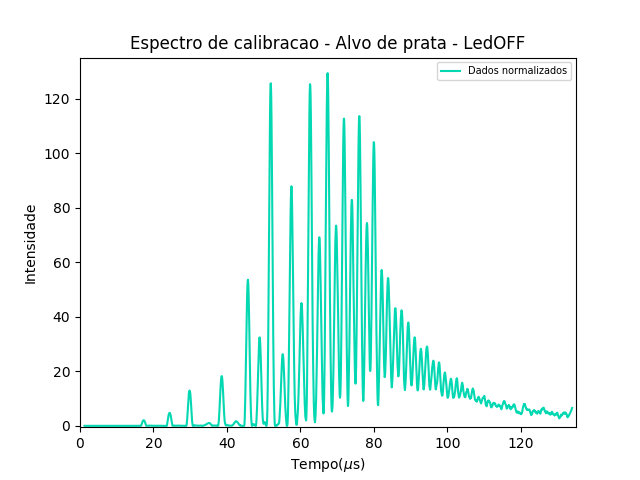
\includegraphics[width=0.7\textwidth]{exp_04/LEDOFF_normalizado_mcp.png}
  \caption{IV- Espectro de calibração com tratamento de dados.}
  \label{fig:04_ledoff_dados_tratados} 
\end{figure}

\begin{figure}
  \centering  
  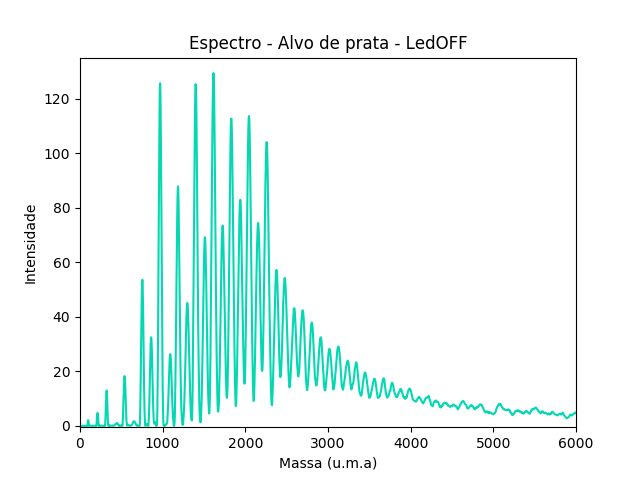
\includegraphics[width=0.7\textwidth]{exp_04/LEDOFF_espec_calib_ag_massa.png}
  \caption{IV- Espectro de calibração com tratamento de dados.}
  \label{fig:04_ledoff_massa} 
\end{figure}



\begin{figure}
  \centering  
  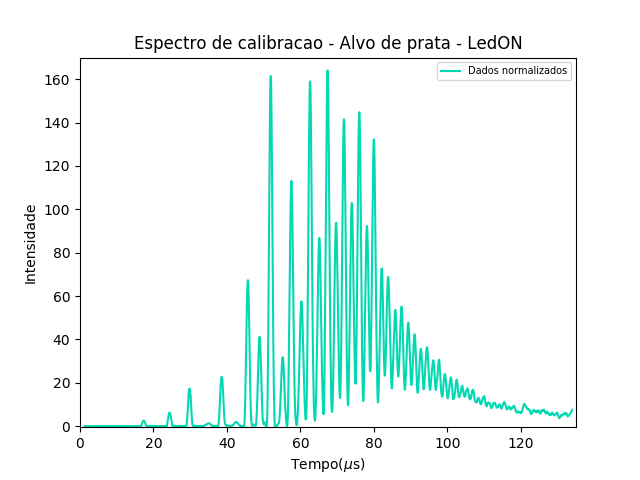
\includegraphics[width=0.7\textwidth]{exp_04/LEDON_normalizado_mcp.png}
  \caption{IV- Espectro de calibração com tratamento de dados.}
  \label{fig:04_ledon_dados_tratados} 
\end{figure}

\begin{figure}
  \centering  
  \includegraphics[width=0.7\textwidth]{exp_04/LEDON_espec_calib_ag_massa.png}
  \caption{IV- Espectro de calibração com tratamento de dados.}
  \label{fig:04_ledon_massa} 
\end{figure}






%\chapter{Conclusões} \label{conclusões}


%% \bibliography{./nsav}
%% \bibliographystyle{unsrt}
\addcontentsline{toc}{chapter}{Bibliografia}
\bibliographystyle{acm}
\bibliography{references.bib}


%\chapter*{Apêndices}
%\markboth{Apêndices}{Apêndices}
%\addcontentsline{toc}{chapter}{Apêndices}


%\appendix
%\title{Apêndices}

%\chapter{Condições de contorno}

%Para simular o hélio nas fases líquida e sólida nas densidades estudadas, utilizamos uma caixa de simulação com 64 ou 108

%\section{Janzen e colaboradores - $V_{pr}$}

%Os valores dos parâmetros para este potencial são os mesmos que para o 

\end{document}


